\documentclass[10pt,a4paper]{report}
\usepackage[utf8]{inputenc}
\usepackage[T1]{fontenc}
\usepackage{amsfonts}
\usepackage{setspace}
\usepackage{graphicx}
\usepackage{array}
\usepackage{fancyhdr}
\usepackage{geometry}
\usepackage{ragged2e}
\usepackage{color}
\usepackage[maxbibnames=99]{biblatex}
\usepackage{tabularx}
\usepackage{float}
\usepackage{listings}
\usepackage{xcolor}

\lstset{
  basicstyle=\ttfamily\small,
  keywordstyle=\color{blue},
  stringstyle=\color{red},
  commentstyle=\color{gray},
  showstringspaces=false,
  breaklines=true,
  frame=single,
  captionpos=b,
  columns=fullflexible,
  upquote=true
}

\addbibresource{reference.bib}

\geometry{
a4paper,
left=1.15in,
right=1.0in,
top=1.0in,
bottom=1.0in,
}

\begin{document}

\pagestyle{empty}

%%%%%%%%%%%%%%%%%%% Front Page  %%%%%%%%%%%%%%%%%%%%%%%
\begin{center}
{\large \textbf{Visvesvaraya Technological University, Belagavi – 590018}}
\begin{figure}[hbtp]
\centering

\includegraphics[width=2.3cm,height=3cm]{./pic/vtu}
\end{figure}

\textbf{MAJOR PROJECT PHASE I REPORT}
\par
\textbf{ON}
\par
\vspace{6pt}
{\Large \textbf{AutoVue: Smart Vehicle ECU Monitoring and Predictive Maintenance}}
\par
\vspace{12pt}
\par
\textit{\textbf{Submitted in partial fulfillment for the award of degree of}}
\par
\vspace{12pt}
\large \textbf{BACHELOR OF ENGINEERING }
\par
\textbf{in}
\par
\large \textbf{ARTIFICIAL INTELLIGENCE AND MACHINE LEARNING}
\par
\vspace{12pt}
\textit{\textbf{Submitted by}}

\begin{center}
\begin{tabular}{l@{\hspace{2cm}}r}
\textbf{\large Anish V S } & \textbf{4SO23AI012} \\
\textbf{\large S K Saichaand Shetty} & \textbf{4SO23AI058} \\
\textbf{\large Yojan D } & \textbf{4SO23AI069} \\
\textbf{\large Pratham U} & \textbf{4SO23AI070} \\
\end{tabular}
\end{center}

\vspace{12pt}
\textit{\textbf{Under the Guidance of}}
\par
\vspace{6pt}
\textbf{Dr Saleena T S }
\par
\vspace{2pt}
\normalsize {Assistant Professor Grade II, Department of ICBS }
\par
\begin{figure}[hbtp]
\centering

\includegraphics[scale=0.6]{./pic/sjeclogo}
\end{figure}
\large \textbf{DEPT. OF INTELLIGENT COMPUTING AND BUSINESS SYSTEMS }
\par \Large \textbf{ST JOSEPH ENGINEERING COLLEGE}
\par
\textbf{An Autonomous Institution}
\par
{\large{(Affiliated to VTU Belagavi, Recognized by AICTE, Accredited by NBA)}}
\par
{\large \textbf{Vamanjoor, Mangaluru - 575028, Karnataka}}
\par
{\Large \textbf{2025-26}}
\end{center}
\newpage

%%%%%%%%%%%%%%%%%%%%%%%%%% Certificate Page %%%%%%%%%%%%%%%
\begin{center}
\LARGE \textbf{ST JOSEPH ENGINEERING COLLEGE}
\par
\Large \textbf{An Autonomous Institution}
\par \large{(Affiliated to VTU Belagavi, Recognized by AICTE, Accredited by NBA)}
\par \vspace{3pt}
\large \textbf{Vamanjoor, Mangaluru - 575028, Karnataka}
\par \vspace{12pt}
\par
\large \textbf{DEPT. OF INTELLIGENT COMPUTING AND BUSINESS SYSTEMS}
\par
\begin{figure}[hbtp]
\centering

\includegraphics[scale=0.5]{./pic/sjeclogo}
\end{figure}


\color{blue}
{\Large \textbf{CERTIFICATE}}
\end{center}
\color{black}
\justifying
\par
\setstretch{1.2}
\noindent

\large
Certified that the project work entitled \textbf{``AutoVue: Smart Vehicle ECU Monitoring and Predictive Maintenance''} carried out by\vspace{2pt}
\par
\noindent
\begin{center}
\begin{tabular}{l@{\hspace{2cm}}r}
\color{blue}
\color{blue}\textbf{Anish V S } & \color{blue}\textbf{4SO23AI012} \\
\color{blue}\textbf{S K Saichaand Shetty} & \color{blue}\textbf{4SO23AI058} \\
\color{blue}\textbf{Yojan D } & \color{blue}\textbf{4SO23AI069} \\
\color{blue}\textbf{Pratham U } & \color{blue}\textbf{4SO23AI070} \\

\end{tabular}
\end{center}
\noindent
the bonafide students of VII semester Artificial Intelligence and Machine Learning in partial fulfillment for the award of Bachelor of Engineering in Artificial Intelligence and Machine Learning of the Visvesvaraya Technological University, Belagavi during the year 2026-2027. It is certified that all suggestions indicated during internal assessment have been incorporated in the report. The project report has been approved as it satisfies the academic requirements in respect of project work prescribed for the said degree.

\par
\vspace{0.55in}
\setstretch{1.15}

\begin{tabularx}{0.95 \textwidth} {
   >{\raggedright\arraybackslash}X
   >{\centering\arraybackslash}X
   >{\raggedleft\arraybackslash}X  }
     \textbf{Dr Saleena T S} & \textbf{Dr Harivinod N} &  \textbf{Dr Rio D'Souza}\\
     Project Guide &  HOD-ICBS & Principal \\
\end{tabularx}


\hspace{7.5cm}
\begin{center}
\large \textbf{External Viva}:
\end{center}
\begin{flushleft}
Examiner's Name
\hspace{7.5cm}
Signature with Date
\end{flushleft}


\begin{flushleft}
1. \ldots\ldots\ldots\ldots\ldots\ldots \ldots \hspace{5.8cm}\ldots\ldots\ldots\ldots \ldots\ldots\ldots
\par
\vspace{0.1in}
2. \ldots\ldots\ldots\ldots\ldots\ldots \ldots \hspace{5.8cm}\ldots\ldots\ldots\ldots \ldots\ldots\ldots
\end{flushleft}
\newpage

%%%%%%%%%%%%%%%%%%%%%% Declaration Page  %%%%%%%%%%%%%%%%%
\centering
\LARGE \textbf{ST JOSEPH ENGINEERING COLLEGE}
\par
\Large \textbf{An Autonomous Institution}
\par \large{(Affiliated to VTU Belagavi, Recognized by AICTE, Accredited by NBA)}
\par \vspace{3pt}
\large \textbf{Vamanjoor, Mangaluru - 575028, Karnataka}
\par \vspace{12pt}  
\par
\large \textbf{DEPT. OF INTELLIGENT COMPUTING AND BUSINESS SYSTEMS}
\par
\begin{figure}[hbtp]
\centering

\includegraphics[scale=0.5]{./pic/sjeclogo}
\end{figure}

\begin{center}
{\textbf{DECLARATION}}
\end{center}
\justifying
\par
\setstretch{1.2}
\fontsize{12}{0}

\noindent We hereby declare that the entire work embodied in this Project Report titled
\textbf{``AutoVue: Smart Vehicle ECU Monitoring and Predictive Maintenance''} has been carried out by us at St Joseph Engineering College, Mangaluru under the supervision of \textbf{Dr Saleena T S,} for the award of \textbf{Bachelor of Engineering} in \textbf{Artificial Intelligence and Machine Learning }. This report has not been submitted to this or any other University  for the award of any  other degree. \\
\vspace{0.25in}

\setstretch{1.75}

\begin{tabular}{l@{\hspace{2cm}}l@{\hspace{2cm}}r}
\textbf{Name } & \textbf{USN} & \textbf{Signature}\\
Anish V S  & 4SO23AI012 & \\
S K Saichaand Shetty & 4SO23AI058 & \\
Yojan D & 4SO23AI069 & \\
Pratham U  & 4SO23AI070 & \\
\end{tabular}

%%%%%%%%%%%%%%%%%%%%%%%% Acknowledgement %%%%%%%%%%%%%%%%%
\newpage
\setstretch{1.2}
\chapter*{Acknowledgement}
\addcontentsline{toc}{chapter}{\numberline{}Acknowledgement}

We dedicate this page to acknowledge and appreciate all those who contributed to the shaping and successful completion of this project. Without their guidance and assistance, the experience of undertaking this work would not have been as smooth and efficient.
\par
\vspace{0.15in}
\noindent We sincerely acknowledge our Project Guide and Project Coordinator, \textbf{Dr. Saleena T. S.}, Assistant Professor Grade II, Department of ICBS, for her valuable guidance, constructive suggestions, and consistent encouragement, which greatly helped us in completing this project successfully.
\par
\vspace{0.15in}
\noindent We owe a profound appreciation to \textbf{Dr. Harivinod N}, Head of the Department, ICBS, whose kind guidance and support contributed significantly to the successful completion of this work.
\par
\vspace{0.15in}
\noindent We are extremely thankful to our Principal, \textbf{Dr. Rio D’Souza}, Director, \textbf{Rev. Fr. Wilfred Prakash D’Souza}, and Assistant Director, \textbf{Rev. Fr. Kenneth Rayner Crasta}, for their constant support and encouragement.
\par
\vspace{0.15in}
\noindent We would also like to acknowledge all the \textbf{faculty members and staff of the Department of ICBS} for their valuable suggestions, guidance, and encouragement throughout the project.
\par
\vspace{0.15in}
\noindent We also extend our sincere appreciation to our \textbf{friends and family members} for their continuous support and encouragement.

%%%%%%%%%%%%%%%%%%%%%%%% Abstract %%%%%%%%%%%%%%%%%
\chapter*{Abstract}
\addcontentsline{toc}{chapter}{Abstract}

\justifying
\setstretch{1.3}

Modern vehicles are equipped with a network of electronic control units (ECUs) and sensors that continuously monitor engine performance, emissions, and overall vehicle health, and this data is accessible through the standard On-Board Diagnostics (OBD-II) interface. However, in most consumer vehicles this data is used only for post-failure fault diagnosis, while the driver receives little or no intelligent interpretation of the vehicle's evolving condition.

This project presents \textbf{AutoVue}, an intelligent vehicle telemetry and diagnostics platform that bridges this gap through two tightly integrated components. The first is a deployable \textbf{FastAPI backend service} that combines an ML-powered diagnostics API with an \textbf{OBD-II data simulator}. The simulator plays back recorded vehicle datasets row by row in real time over REST and WebSocket channels, so that the entire platform can be demonstrated, tested, and validated without a physical vehicle. The second component is a high-performance \textbf{Android telemetry cockpit application} built with Jetpack Compose, which renders live engine instrumentation, multi-channel waveform oscilloscopes, GPS trip mapping, and diagnostic trouble code (DTC) management.

Three machine learning models run automatically on every telemetry tick: an \textbf{XGBoost classifier} that profiles driver behaviour as Economical, Moderate, or Aggressive from rolling telemetry windows; a \textbf{PyTorch LSTM Autoencoder} that detects vehicle health anomalies by learning normal correlations between ten OBD-II sensor features and flagging broken relationships before failure occurs; and a \textbf{three-tier physics-based fuel estimator} that computes instantaneous fuel consumption and mileage from Mass Air Flow, Manifold Absolute Pressure, and throttle heuristics. A smart alert engine with Text-to-Speech announcements, sensor override dials for live demonstrations, GPS route integration, and a DTC scanner with a digital service ticket system complete the platform.

The system is validated end-to-end using bundled normal and anomaly driving datasets, demonstrating that affordable, non-intrusive, standards-based predictive maintenance is achievable on consumer hardware, and laying the foundation for future composite health scoring and remaining-useful-life forecasting.

\newpage

\pagestyle{plain}
\tableofcontents
\listoffigures
\listoftables
\newpage

%---------------------------- Chapter ONE --------------------------
\chapter{Introduction}
\par
\section{Background}

Modern vehicles are equipped with a wide range of electronic control units (ECUs) and embedded sensors that continuously monitor engine performance, emissions, safety, and overall vehicle health. These sensors generate valuable diagnostic and operational data, which can be accessed through the On-Board Diagnostics (OBD-II) interface. However, in most consumer vehicles, this data is primarily used for fault diagnosis after a failure has already occurred, rather than for proactive monitoring or early prediction of issues.
\par
Traditional vehicle maintenance practices rely on fixed service intervals or manual inspection, which may lead to unnecessary maintenance or delayed detection of critical faults. With the increasing availability of vehicle sensor data and advancements in machine learning, there is a strong opportunity to shift from reactive maintenance to predictive and condition-based maintenance. Realising this vision in practice, however, requires more than accurate models: it requires a complete, deployable pipeline from raw sensor stream to a driver-facing interface, together with a practical way to develop and demonstrate such a system without permanently instrumenting a vehicle.
\par
This project proposes and implements \textbf{AutoVue}, an Intelligent Vehicle Telemetry and Diagnostics Platform that addresses both concerns. A deployable FastAPI backend service hosts three specialised machine learning models and an integrated OBD-II simulator that plays back recorded vehicle datasets in real time over REST and WebSocket channels, while a native Android application built with Jetpack Compose provides a high-performance digital cockpit for live engine instrumentation, machine-learning insights, GPS trip mapping, and diagnostic fault management.

\section{Problem Statement}

Although modern vehicles generate large volumes of diagnostic and sensor data through onboard ECUs, this data is underutilized in consumer vehicles. Existing OBD-II tools mainly display raw sensor values or diagnostic trouble codes (DTCs) without providing intelligent interpretation, trend analysis, or predictive insights. At the same time, developing and demonstrating an intelligent monitoring system traditionally requires a physical vehicle and a wired OBD-II adapter at all times, which constrains development, testing, and live presentation. Hence, there is a need for an intelligent system that integrates OBD-II data acquisition with machine learning techniques to enable real-time vehicle health monitoring and predictive maintenance, together with a realistic data source that allows the full pipeline to be exercised without a vehicle.

\section{Scope}

The scope of this project encompasses the full pipeline from vehicle data acquisition to intelligent insight delivery. The system performs data acquisition from standard OBD-II PIDs supported by most passenger vehicles, enabling real-time monitoring of key engine and vehicle health parameters. Because the current implementation is validated through a dataset-driven simulator that reproduces real OBD-II recordings row by row, the same pipeline that serves simulated data can later be pointed at a physical ELM327 adapter without changes to the machine learning models, the API layer, or the mobile application. All results, including driver behaviour classification, health anomaly alerts, fuel estimates, and diagnostic trouble codes, are presented through a native Android cockpit application backed by a browser-based control dashboard.
\par
The project operates within well-defined boundaries to ensure practical feasibility. Data access is strictly non-intrusive, relying solely on read-only OBD-II communication without modifying any vehicle systems. The scope is limited to consumer-grade passenger vehicles that expose standard OBD-II PIDs, excluding proprietary manufacturer ECU protocols. The machine learning scope covers driver behaviour classification, multivariate health anomaly detection, and physics-based fuel consumption estimation; composite health scoring and remaining-useful-life forecasting are identified as future extensions. The system is developed and validated as a prototype using bundled recorded driving datasets rather than a large-scale commercial deployment.
\par
The applications of this system are broad and practically significant. It can serve individual vehicle owners seeking proactive health monitoring, fleet operators requiring centralized diagnostic insights, used-car dealers performing vehicle condition assessments, and driver assistance platforms looking to integrate intelligent health alerts into their offerings. The simulator-backed architecture additionally makes the platform a practical teaching and demonstration tool for automotive machine learning.

%---------------------------- Chapter TWO --------------------------

\chapter{Literature Survey}
\section{Introduction}

This chapter reviews the existing body of research at the intersection of OBD-II vehicle data, machine learning, and predictive maintenance. The survey examines twelve representative works spanning fuel consumption estimation, driver behaviour classification, engine health monitoring, anomaly and fault detection, and in-vehicle data architectures. Each work is analysed for the problem it addresses, the machine learning approach adopted, its demonstrated strengths, and the gaps it leaves open. The chapter concludes with a comparative synthesis that motivates the design of AutoVue.

\section{A Review of OBD-II-Based Machine Learning Applications for Sustainable, Efficient, Secure, and Safe Transportation}

Michailidis et al. (2025) \cite{article1} present a holistic cross-domain review of OBD-II-based machine learning applications for sustainable, efficient, secure, and safe transportation. The survey consolidates approaches based on supervised learning, deep learning, and reinforcement learning applied to vehicle telemetry. Its principal strength is the breadth of the synthesis, which maps how fragmented research strands relate to one another; however, as a survey it contributes no new experimental results or deployable system. This work establishes the landscape into which AutoVue positions itself, and highlights that few reviewed systems progress from algorithmic results to a functioning end-to-end platform.

\section{A Modular In-Vehicle C-ITS Architecture for Sensor Data Collection, Vehicular Communication, and Data Transmission}

Rocha et al. (2023) \cite{article2} propose a modular in-vehicle Cooperative Intelligent Transport Systems (C-ITS) architecture for sensor data collection, vehicular communication, and data transmission. The architecture demonstrates a clean, modular separation of concerns for in-vehicle data pipelines and achieves scalable data collection through sensor fusion. Its identified weakness is the absence of any machine learning interpretation layer: data is collected and transmitted, but never converted into diagnostic insight. AutoVue adopts the same modular philosophy in its FastAPI backend while adding the missing ML inference stage that consumes the collected telemetry.

\section{Design of Onboard Vehicle Diagnosis Fault Monitoring System using IoT and Machine Learning}

Anil et al. (2021) \cite{article3} design an onboard vehicle diagnosis and fault monitoring system using IoT and machine learning, motivated by the high cost of professional scan tools. The system couples low-cost IoT hardware with Ridge regression, LASSO, and a neural network to monitor vehicle condition at an affordable price point. The work demonstrates that diagnostic intelligence can be delivered without proprietary garage equipment, but relies on add-on external sensors rather than the vehicle's own ECU data, limiting the richness of the observed vehicle state. AutoVue follows the low-cost, non-intrusive philosophy but sources all parameters directly from the standard OBD-II PID set.

\section{Fuel Consumption Using OBD-II and Support Vector Machine Model}

Abukhalil et al. (2020) \cite{article4} estimate fuel consumption using OBD-II parameters and a Support Vector Machine model, addressing the difficulty of modelling Mass Air Flow based fuel complexity. The SVM model achieves a strong 2.436 RMSE accuracy figure, demonstrating that classic kernel methods remain competitive for fuel estimation. The principal limitation is the use of a small dataset collected on a single route, which constrains generalisation. AutoVue's fuel module instead adopts a physics-first strategy — a three-tier estimator anchored in the MAF speed-density relationship — which requires no retraining to adapt to a new vehicle, and is complemented rather than replaced by learned models.

\section{Revving Up Insights: Machine Learning-Based Classification of OBD II Data and Driving Behaviour}

Singh \& Sharma (2025) \cite{article5} classify OBD-II data and driving behaviour using Random Forest, K-Nearest Neighbours, and AdaBoost, targeting the detection of risky driving patterns. The reported behaviour-classification accuracy reaches 100\%, the strongest figure in the surveyed literature. However, perfect accuracy on a limited corpus carries a significant risk of overfitting, and the study does not model driving context or temporal windows. AutoVue's driver behaviour module addresses this by classifying over rolling time-series windows of telemetry with engineered statistical features, a design that is inherently more robust to overfitting on isolated samples.

\section{Study of Machine Learning Based Applications on OBD-II Port by Using Internet of Vehicles}

Patil et al. (2019) \cite{article6} study machine learning applications on the OBD-II port within an Internet of Vehicles (IoV) gateway prototype, aiming at affordable road safety. The proposed gateway applies decision-tree methods including J48 and AdaBoost, but remains a proposal: no experimental results or live demonstration are reported. The work is nonetheless influential in framing the OBD-II port as an accessible, standardised gateway for consumer vehicle intelligence — the premise on which AutoVue's simulator-backed architecture is built.

\section{Trip-Wise Driver Behavior Analysis and Vehicle Health Recommendation System using Machine Learning}

Singhai \& Mehta (2026) \cite{article12} develop a trip-wise driver behavior analysis and vehicle health recommendation system using machine learning, built on a lightweight web framework with logistic regression. Its strength is the integration of driver feedback and vehicle recommendations in one lightweight pipeline. The principal gap is that analysis is performed post-trip only: no real-time insight is available to the driver while driving. AutoVue closes this loop by running the same class of analysis continuously on a rolling buffer and streaming results to the driver over a WebSocket within the second they are computed.

\section{Enhancing predictive maintenance in automotive industry: addressing class imbalance using XGBoost and LightGBM}

Mahale et al. (2025) \cite{article7} enhance predictive maintenance in the automotive industry by addressing class imbalance using XGBoost and LightGBM with SMOTE resampling. The work demonstrates that gradient-boosted ensembles effectively handle the rare-fault problem, where genuine failures are vastly outnumbered by normal operation. The limitation is an engine-only focus with no treatment of noisy real-world streams. AutoVue's health module takes a complementary approach to the same rare-fault problem: rather than classifying labelled faults, an LSTM Autoencoder learns the manifold of normal multivariate sensor behaviour and flags any departure from it, which requires no failure labels at all.

\section{Driving behavior analysis and classification by vehicle OBD data using machine learning}

Kumar \& Jain (2023) \cite{article8} analyse and classify driving behavior from vehicle OBD data using Random Forest, AdaBoost, and SVM. A notable strength is that the approach requires no hardware modification and exploits more than fifty PIDs. Validation, however, is restricted to a single vehicle. The work reinforces the surveyed consensus that tree-based ensembles are the strongest performers on tabular OBD-II data — a finding that directly informed AutoVue's choice of XGBoost for driver behaviour classification.

\section{Machine Learning for Real-Time Fuel Consumption Prediction and Driving Profile Classification}

Canal et al. (2024) \cite{article9} apply machine learning for real-time fuel consumption prediction and driving profile classification, evaluating XGBoost, Support Vector Regression, and NARX architectures against real-time ECU data. The study reports an excellent 0.99 $R^2$ efficiency score, while observing a high failure rate of deep learning models on this task relative to boosted trees. AutoVue's design is consistent with this empirical conclusion: its production fuel path is a transparent physics estimator, while its driver profiling uses the XGBoost family that the literature repeatedly validates.

\section{Utilizing AI for predictive maintenance and problem resolution to optimize technical support processes}

Folorunsho et al. (2024) \cite{article10} examine the utilisation of AI for predictive maintenance and problem resolution in optimising technical support processes, through a collection of industrial AI case studies. The work documents maintenance-related downtime reductions approaching 50\%, quantifying the economic value of predictive strategies. Its limitation is the high deployment cost of industrial-scale solutions. AutoVue targets the same predictive value at the opposite end of the cost spectrum: a free-tier cloud deployment of a single FastAPI service plus a consumer Android phone.

\section{Data-Driven Engine Health Monitoring with AI}

Hornyák (2024) \cite{article11} presents data-driven engine health monitoring using AdaBoost, demonstrating an architecture-agnostic monitoring approach that is not tied to a specific engine family. Reported accuracy reaches 80\%, and the work is weakened by its reliance on theoretical rather than extensively road-validated data. The study supports AutoVue's guiding principle that monitoring should depend only on standardised PIDs so that it generalises across passenger vehicles.

\section{Comparison of Related Work}

\begin{table}[H]
\centering
\caption{Comparison of Existing OBD-II and ML-Based Vehicle Monitoring Systems}
\setstretch{1.0}
\renewcommand{\arraystretch}{1.5}
\small
\begin{tabularx}{\textwidth}{|l|l|X|l|X|X|}
\hline
\textbf{\#} & \textbf{Paper} & \textbf{Problem Addressed} & \textbf{ML Model} & \textbf{Strengths} & \textbf{Gap Identified} \\ \hline
1 & Abukhalil et al. (2020) \cite{article4} & MAF-based fuel complexity & SVM & 2.436 RMSE accuracy & Small dataset, single route \\ \hline
2 & Anil et al. (2021) \cite{article3} & High cost of scan tools & Ridge, LASSO, NN & Low-cost IoT solution & Add-on sensors only \\ \hline
3 & Canal et al. (2024) \cite{article9} & Real-time ECU fuel prediction & XGBoost, SVR, NARX & 0.99 R2 score efficiency & High DL failure rate \\ \hline
4 & Folorunsho et al. (2024) \cite{article10} & Industrial maintenance opt. & AI Case Studies & 50\% downtime reduction & High deployment cost \\ \hline
5 & Horny\'ak (2024) \cite{article11} & Scalable engine monitoring & AdaBoost & Arch-agnostic monitoring & Theoretical data, 80\% accuracy \\ \hline
6 & Kumar \& Jain (2023) \cite{article8} & Driving behavior sig. & RF, AdaBoost, SVM & No hardware change (50+ PIDs) & Single vehicle validation \\ \hline
7 & Mahale et al. (2025) \cite{article7} & Failure class imbalance & XGBoost, LightGBM & Handles rare faults (SMOTE) & Engine only, no noisy streams \\ \hline
8 & Michailidis et al. (2025) \cite{article1} & Fragmented research synthesis & Supervised, DL, RL & Holistic x-domain review & Survey only, no new results \\ \hline
9 & Patil et al. (2019) \cite{article6} & Affordable road safety & AdaBoost, J48 & IoV gateway prototype & Proposal only, no results \\ \hline
10 & Rocha et al. (2023) \cite{article2} & Scalable C-ITS framework & Sensor Fusion & Modular architecture & No ML interpretation \\ \hline
11 & Singh \& Sharma (2025) \cite{article5} & Risky behavior detection & RF, KNN, AdaBoost & 100\% behavior accuracy & Overfitting risk, no context \\ \hline
12 & Singhai \& Mehta (2026) \cite{article12} & Trip-wise integrated alerts & Logistic Regression & Lightweight web framework & Post-trip only analysis \\ \hline
\end{tabularx}
\end{table}

\section{Proposed System}
The current landscape of vehicle diagnostics is transitioning from exclusive, proprietary service-center tools to a democratised model built on the OBD-II standard. While the raw data and analytical techniques surveyed above are mature, there remains a significant gap in synthesising them into a complete, deployable, user-facing system for everyday drivers — and, just as importantly, a practical way to build and demonstrate such a system without permanently instrumenting a vehicle. This project bridges both gaps through \textbf{AutoVue}, an intelligent vehicle telemetry and diagnostics platform consisting of a deployable FastAPI backend service with an integrated OBD-II simulator, and a native Android cockpit application. \par

The backend's multi-dimensional data acquisition strategy reads a high-density parameter set from recorded real driving sessions — engine RPM, vehicle speed, coolant temperature, intake air temperature, manifold absolute pressure, mass air flow, throttle and accelerator pedal positions, and ambient temperature — and replays them row by row in real time over REST and WebSocket channels. Because the simulator emits the exact standard sensor field contract used throughout the system, the same pipeline can later be pointed at a physical ELM327 adapter without touching the machine learning models, the API layer, or the mobile application. \par

At its core, the system runs a machine learning pipeline of three specialised models on a rolling telemetry buffer. An \textbf{XGBoost classifier} profiles driver behaviour as Economical, Moderate, or Aggressive with a confidence score and a coaching message; a \textbf{PyTorch LSTM Autoencoder} learns the normal correlations between ten OBD-II sensor features and flags anomalies — such as high RPM accompanied by abnormally low airflow — before they manifest as failures, reporting per-feature reconstruction errors and the specific triggered sensors; and a \textbf{three-tier physics-based fuel estimator} computes instantaneous fuel consumption from Mass Air Flow, falling back to a speed-density calculation and then a throttle heuristic, yielding consumption rate, mileage, and trip cost. \par

The platform addresses a critical need for road safety and economic efficiency, particularly in regions like India where maintenance is often reactive rather than proactive. An affordable, non-intrusive monitoring system using the standard OBD-II data available in virtually all modern passenger vehicles can reduce unexpected breakdowns, extend vehicle longevity, and lower costs for individual owners and fleet operators alike. \par

The novelty of the work lies in its integration of capabilities that the surveyed studies handled only in isolation, delivered as a single deployable unit: real-time telemetry streaming with automatic ML inference attached to every tick, an interactive OBD-II simulator with sensor override dials and dataset switching for reproducible live demonstrations, a diagnostic trouble code scanner with a digital service ticket workflow, GPS route integration for trip replay, and a driver-facing Android cockpit with analog-digital instrumentation, waveform oscilloscopes, and spoken alerts. Unlike previous prototypes tied to specific vehicle models or external sensor rigs, AutoVue's reliance on the standardised OBD-II field contract ensures broad generalisability, while its simulator-first architecture makes every result reproducible without a vehicle present. \par

%---------------------------- Chapter THREE --------------------------

\chapter{Software Requirements Specification}
\section{Introduction}

AutoVue is developed to provide a proactive, data-driven approach to vehicle diagnostics and maintenance management. Modern vehicles are equipped with On-Board Diagnostics II (OBD-II) systems that generate continuous streams of operational data related to engine performance, emissions, and overall vehicle health. While conventional diagnostic tools primarily detect faults after they occur, this project transforms raw vehicle data into intelligent insights capable of flagging abnormal behaviour before it becomes critical. By integrating real-time OBD-II telemetry with machine learning inference and a native Android cockpit, the system enhances reliability, safety, and maintenance efficiency. \par

The system collects essential vehicle parameters — engine RPM, vehicle speed, coolant temperature, intake air temperature, manifold absolute pressure, mass air flow, throttle position, ambient temperature, and accelerator pedal positions — acquired in real time directly from the vehicle's Engine Control Unit (ECU) via a Bluetooth OBD-II adapter. These parameters are processed by a driver behaviour classifier, a health anomaly detector, and a physics-based fuel estimator to identify irregular patterns and quantify consumption. The results are presented through a high-performance Android application that displays live instrumentation, machine-learning insights, GPS trip mapping, and diagnostic trouble code (DTC) management in a clear, driver-friendly format. \par

This Software Requirements Specification (SRS) document defines the functional and non-functional requirements of the system as implemented. It establishes system boundaries, operational constraints, and user interaction guidelines. The system is implemented as a prototype focused on passenger vehicles supporting standard OBD-II PIDs, operating in a non-intrusive read-only mode, and validated through live acquisition from the vehicle's OBD-II port using an ELM327-compatible Bluetooth adapter. The overall objective is to reduce unexpected breakdowns, minimize repair costs, extend vehicle lifespan, and contribute to intelligent transportation and smart mobility solutions.

\section{Functional requirements}
This section specifies the functional requirements of AutoVue. The requirements are derived from the identified research gaps in the surveyed literature and the implemented capabilities of the platform. Each requirement is described in terms of input, processing, and output.

\subsection{Real-Time OBD-II Telemetry Streaming}
The system shall stream live OBD-II parameter values to connected clients in real time. Streaming shall be provided over a secure WebSocket channel (\texttt{/api/ws/live}), with an automatic REST polling fallback to a latest-snapshot endpoint (\texttt{/api/live-data}). At minimum, the streamed parameters shall include vehicle speed (VSS), engine RPM, throttle position, engine coolant temperature, intake air temperature, calculated engine load, barometric/ambient temperature, manifold absolute pressure (MAP), and mass air flow (MAF). The system shall also display the active OBD-II protocol and the measured telemetry throughput rate. \par

\subsection{OBD-II Adapter Connection and Acquisition Control}
The system shall discover, pair with, and connect to an ELM327-compatible Bluetooth OBD-II adapter installed in the vehicle's diagnostic port. The system shall auto-detect the active OBD-II protocol (e.g. ISO 15765-4 CAN) upon connection, and shall provide control endpoints to initiate, pause, resume, and terminate a live acquisition session. The system shall report live connection status including adapter connection state, active protocol, session duration, and current telemetry throughput rate, and shall attempt automatic reconnection on an unexpected adapter disconnection. \par

\subsection{Machine Learning Inference on Live Telemetry}
The system shall execute three machine learning models automatically on a rolling buffer of the most recent telemetry ticks, and shall attach inference results to every streamed tick under an \texttt{ml} key. \par
\begin{itemize}
  \item \textbf{Driver behaviour classification:} an XGBoost model shall classify driving style as Economical, Moderate, or Aggressive from a rolling window of RPM, speed, and throttle arrays (minimum 5 points, active from tick 30), returning a confidence score, a coaching message suitable for text-to-speech, and the nine engineered statistical features used.
  \item \textbf{Vehicle health anomaly detection:} an LSTM Autoencoder shall evaluate the most recent 24 ticks across ten sensor features (active from tick 24), returning an anomaly flag, an anomaly score, per-feature reconstruction errors, and the list of triggered features whose errors exceed their individual thresholds.
  \item \textbf{Fuel consumption estimation:} a three-tier physics engine shall compute the fuel consumption rate (g/s) and instantaneous mileage (km/L) from the most recent 20 ticks (active from tick 20), using a MAF-based method as Tier 1, a speed-density calculation using MAP and RPM as Tier 2, and a throttle heuristic as Tier 3, with the engine-off case handled as Tier 0.
\end{itemize}
The same inference capabilities shall also be exposed as standalone REST endpoints (\texttt{/api/driver/predict}, \texttt{/api/health/predict}, \texttt{/api/fuel/predict}) so that the models can be exercised independently of the live stream. \par

\subsection{Diagnostic Trouble Code (DTC) Management}
The system shall support injection of OBD-II Diagnostic Trouble Codes into the live stream through REST endpoints: listing active codes, replacing the active code list (auto-uppercased), clearing all codes, and removing a specific code. Codes spanning the powertrain (P), chassis (C), body (B), and network (U) domains shall be supported. When codes are active, the broadcast payload shall include a \texttt{dtcs} array; when cleared, the key shall be omitted so that existing consumers remain unaffected. The Android application shall decode codes with symptom explanations and severity ratings, and shall support automatic or manual creation of digital service tickets stamped with vehicle VIN, mileage, and fault description, with dispatch integration to service partners or Telegram notifications. \par

\subsection{GPS Route Integration}
The system shall acquire GPS position, elevation, bearing, and speed directly from the Android device's onboard GPS sensor in real time, and shall fuse each GPS sample with the concurrently streamed OBD-II tick using timestamp alignment. Every streamed tick shall include the GPS fields, and the system shall expose a full-route polyline endpoint (\texttt{/api/route}) and a trip summary endpoint (\texttt{/api/trip-summary}) returning distance, average and maximum speed, and average RPM and throttle. Sessions without a valid GPS fix shall continue to function identically, with GPS endpoints returning a clear not-found response so that frontends can gracefully degrade. \par

\subsection{Alert Engine and Voice Alerts}
The system shall provide a prioritized alert banner with severity tags (CRITICAL, WARNING, INFO) for overspeeding, engine overheating (coolant above 100\,\textdegree{}C), cold-engine revving (coolant below 60\,\textdegree{}C at more than 3500 RPM), and detected sensor anomalies. The Android application shall additionally provide spoken alerts using the Android Text-to-Speech engine, with customizable cooldown debounce and independent toggles for speed, temperature, and anomaly announcements. \par

\subsection{Vehicle Profile Management}
The Android application shall allow users to register and switch between multiple vehicle and driver profiles, captured through a two-page onboarding wizard covering profile name, fuel supply type (gasoline, diesel, hybrid, electric, LPG), start-stop system status, engine displacement, maximum power, odometer reading, curb weight, manufacturer reference consumption, corrective factor, tank capacity, current fuel level, and VIN. Profile parameters shall calibrate the physics-based fuel modelling. \par

\subsection{Trip Logging and Efficiency Tracking}
The Android application shall track trips on an interactive map with switchable display modes (standard path, speed heatmap, driving behaviour overlay, and fuel efficiency trace); maintain a refuelling diary recording fuel quantity, price per litre, total cost, and odometer readings; and implement a start-stop efficiency optimizer that tracks engine shut-off time versus stationary time at idling, computing cumulative fuel and financial savings. \par

\section{Non-Functional Requirements}

This section specifies the non-functional attributes of AutoVue. These requirements define quality standards and operational expectations for the system as deployed.

\subsection{Reliability}
The backend service shall remain stable under continuous live telemetry acquisition from the vehicle ECU, and WebSocket clients shall tolerate transient network interruptions by falling back to REST polling and resuming the stream automatically. Unsupported or missing sensor fields reported by the adapter shall be handled gracefully with default values rather than functional failure. \par

\subsection{Availability}
The backend shall be deployable as a single containerized service on free-tier cloud hosting, with a health-check endpoint (\texttt{/health}) used by the hosting platform to detect a live instance. The Android application shall continue to render its last known state and degrade to REST polling when the live stream is unavailable. \par

\subsection{Scalability}
The system shall maintain a configurable history ring buffer (default 500 ticks) to bound memory use, sized to the ECU's live polling rate. The WebSocket layer shall support multiple concurrently connected clients receiving the same broadcast ticks. \par

\subsection{Security}
All streamed telemetry shall be transported over secure WebSocket (\texttt{wss://}) and HTTPS in deployment. The platform is currently a single-user academic prototype and does not implement authentication; user accounts, JWT-based access control, and bcrypt credential storage are identified as future extensions. \par

\subsection{Maintainability}
The backend shall follow a modular package layout separating machine learning code, ECU acquisition services, and API routes, so that individual components — such as the anomaly detector or the fuel estimator — can be independently retrained, replaced, or extended. The standard ten-field sensor contract shall be the single interface between the OBD-II adapter, ML models, and clients, so that acquisition hardware can be swapped without touching downstream code. \par

\subsection{Portability}
The Android application shall run on devices with Android API levels up to target SDK 34, and its layout engine shall adapt defensively across phone aspect ratios and screen densities. The backend shall be deployable on any platform supporting Python 3.11 and Docker without code changes. \par

\subsection{Usability}
A first-time user shall be able to install the Android application, complete the two-page profile wizard, connect to the telemetry stream using the OBD Link control, and view live instrumentation within minutes using only on-screen guidance. \par

\section{User Interface requirements}
This section describes the logical design and behavioural specification of the user-facing interfaces of AutoVue. The primary user interface is the native Android cockpit application; a browser-based control dashboard ships with the backend for live acquisition administration.

\subsection{Instrument Cluster (Cockpit)}
The primary screen shall be a dual analog-digital instrument cluster rendering a custom canvas-drawn analog speedometer with dynamic sweep needle, a tachometer with an RPM redline threshold, a coolant temperature gauge with cold and overheat zones, and a fuel percentage meter. Instantaneous power (HP) and engine torque (Nm) shall be computed and plotted against peak power and torque RPM curves. A trip computer HUD shall display elapsed trip time, distance, fuel cost, instantaneous and average consumption (L/100km), instantaneous speed, and an eco-driving score. \par

\subsection{Live Telemetry Sensor Grid}
A sensor grid shall present real-time OBD-II parameter values with units and a protocol/telemetry-speed indicator, including at minimum vehicle speed, engine RPM, throttle position, coolant temperature, intake air temperature, engine load, ambient temperature, MAP, and MAF. \par

\subsection{Oscilloscope and Waveform Visualizer}
A diagnostic strip-chart view shall render scrolling, multi-channel waveforms for RPM, speed, intake air temperature, engine load, coolant temperature, MAP, MAF, and accelerator pedal position, styled after professional automotive diagnostic oscilloscopes. The view shall provide pause/resume, zoom scaling, and peak-value indicators. \par

\subsection{Machine Learning Insights Panels}
The interface shall summarize the three ML models: the driver behaviour classification with confidence and coaching recommendation; the health status with anomaly score and triggered features; and the fuel panel with instantaneous consumption rate, mileage, estimated range, and trip cost. \par

\subsection{Alerts, DTCs, and Service Tickets}
An alert banner shall display prioritized notifications with severity tags and shall support spoken Text-to-Speech announcements with per-category toggles and cooldown debounce. A DTC screen shall list scanned codes with decoded descriptions and severity ratings, and shall support creation and dispatch of digital service tickets stamped with VIN, mileage, and fault description. \par

\subsection{Trip Map, Refuelling, and Start-Stop Views}
A GPS map view shall replay the route with switchable overlays (speed heatmap, driving behaviour, fuel efficiency). A refuelling diary shall log quantity, price, cost, and odometer per stop, with low-fuel awareness below 50\,km of estimated range. A start-stop view shall show engine shut-off versus stationary time with cumulative fuel and cost savings. \par

\subsection{OBD Adapter Diagnostics Dashboard (Web)}
The backend shall serve a single-file browser dashboard for monitoring live acquisition: adapter connection status, active protocol, live sensor values, and acquisition session controls (start/pause/resume/stop). \par

\section{Software Requirements }
\subsection{Programming Language}
The backend shall be developed in Python 3.11, serving as the language for acquisition services, machine learning inference, and the API layer. The Android application shall be developed in Kotlin. \par

\subsection{Backend API Framework}
The backend shall be implemented using FastAPI (0.111) with Uvicorn, exposing REST endpoints for machine learning inference, adapter connection control, DTC management, GPS route data, and history retrieval, together with WebSocket endpoints for live telemetry and acquisition logs. \par

\subsection{Machine Learning Frameworks}
The system shall employ XGBoost 2.0 for driver behaviour classification, PyTorch 2.2 for the LSTM Autoencoder health model, and Scikit-learn for feature scaling and threshold management. The fuel estimation module shall be physics-based and require no training. Model artefacts (pickled scalers, thresholds, model weights, and metadata) shall be version-controlled files loaded at startup. \par

\subsection{Networking Libraries}
The Android application shall use the OkHttp WebSocket client for real-time streaming and Retrofit 2 with the Moshi converter for REST calls. The default backend endpoint shall be configurable in the application container. \par

\subsection{Android UI Framework}
The application shall be built with Jetpack Compose using Material Design 3, Kotlin Coroutines, and StateFlow, following a Clean Architecture / MVVM pattern with a responsive layout engine using defensive text truncation and single-line constraints. \par

\subsection{Audio and Accessibility}
The application shall use the Android Text-to-Speech engine for spoken driver alerts. \par

\subsection{Data Processing Libraries}
The backend shall use NumPy and Pandas for telemetry cleaning, missing-value handling, and rolling-window feature extraction. \par

\subsection{Version Control and Development Environment}
Source code shall be managed with Git and hosted on GitHub. Machine learning experimentation shall be conducted in Jupyter Notebook, and the Android application developed in Android Studio. \par

\subsection{Containerization and Deployment}
The backend shall ship with a Dockerfile enabling single-container deployment to cloud platforms such as Render, with environment-variable-based configuration for acquisition settings. \par

\section{Hardware Requirements }
\subsection{OBD-II Data Source}
The primary data source shall be an ELM327-compatible OBD-II adapter connected to the vehicle's diagnostic port and paired with the Android device over Bluetooth. The backend shall acquire live telemetry from this adapter using the python-OBD library over the standard ISO 15765-4 CAN protocol, feeding the same standard field contract consumed by the ML models, API layer, and Android application. \par

\subsection{Android Device}
The Android cockpit application shall target devices running Android with support for API level 34, requiring network connectivity (Wi-Fi or cellular) to reach the backend service. \par

\subsection{Server}
The backend shall be deployable on any host capable of running the container, including free-tier cloud instances with approximately 512\,MB–1\,GB RAM, noting that cold starts on free tiers may take 30–60 seconds. \par

\section{Performance Requirements}

\subsection{Live Telemetry Polling Rate}
The system shall poll the ECU via the OBD-II adapter at a sustained rate of approximately one telemetry tick per second across the standard sensor set. \par

\subsection{Machine Learning Inference Latency}
Inference shall complete within the one-second tick interval for all three models: fuel estimation activates from tick 20, health anomaly detection from tick 24, and driver behaviour classification from tick 30, with results attached to every subsequent tick. \par

\subsection{API Responsiveness}
REST endpoints for live data, history, acquisition control, and ML prediction shall respond interactively (sub-second under nominal load) so that the control dashboard and Android fallback polling remain fluid. \par

\subsection{Resource Bounds}
The history ring buffer shall be capped (default 500 entries) to bound memory consumption, and the live acquisition session shall report tick counts, session duration, and any missing-value or dropped-tick statistics so that data quality issues are visible to the operator. \par

\section{Design Constraints}

\subsection{OBD-II Protocol Limitations}
The system is constrained to the standard OBD-II Mode 01 parameter set for real-time telemetry and standard DTC domains (P, C, B, U). Manufacturer-specific extended PIDs shall not be relied upon for core functionality. \par

\subsection{Standard Sensor Field Contract}
All telemetry — from the OBD-II adapter, the WebSocket stream, REST endpoints, and history — shall use one fixed set of 10 Standard field names. This contract is the stability boundary that allows acquisition hardware and ML code to evolve independently.\par

\subsection{Read-Only ECU Access}
The system shall operate strictly in read-only fashion with respect to the vehicle. The system shall not issue ECU-modifying commands or clear diagnostic codes on the vehicle without explicit user confirmation. \par
\subsection{Internet Dependency}
Full functionality - live streaming, ML inference, and route data - depends on connectivity between the Android application and the hosted backend. The application shall degrade to REST polling and retain its last known state during interruptions. \par

\subsection{Deployment Environment Constraints}
On free-tier hosting, the filesystem is not persistent across redeploys. Cold-start wake-up latency shall be accounted for in live demonstrations. \par

%---------------------------- Chapter FOUR --------------------------

\chapter{System Design}
\section{Abstract Design}
\subsection{Architectural diagram}
The AutoVue architecture follows a layered design pattern comprising four distinct tiers:
Data Source, Backend Service (ML API + Data Acquisition), Transport, and Clients. Each tier has a clearly defined responsibility and communicates through well-specified interfaces. The backend is a single deployable FastAPI process that receives real-time vehicle data via Bluetooth directly from the car's ECU or OBD-II adapter. It runs the three machine learning inference functions automatically on a rolling buffer of incoming ticks, attaching results to every broadcast. This separation of concerns enables independent testing, replacement, and scaling of individual components, and guarantees that the Android client and all ML code depend only on the fixed ten-field sensor contract.

The AutoVue system follows a multi-layer architecture:

\begin{table}[H]
\centering
\renewcommand{\arraystretch}{1.3}
\begin{tabular}{|p{3cm}|p{4cm}|p{6cm}|}
\hline
\textbf{Layer} & \textbf{Technology Stack} & \textbf{Responsibility} \\
\hline

Data Source Layer & OBD-II Bluetooth Adapter, ECU & Real-time acquisition of live driving sessions directly from the vehicle's onboard diagnostics port \\
\hline

Backend Service Layer & Python 3.11, FastAPI, Bluetooth Data Gateway & Tick building, rolling ML buffer, XGBoost / LSTM Autoencoder / physics-fuel inference, DTC state, GPS route data \\
\hline

Transport Layer & WebSocket (\texttt{/api/ws/live}, \texttt{/api/ws/logs}), REST API, HTTPS/WSS & Real-time broadcast of sensor + ML ticks, snapshot/history polling \\
\hline

Client Layer & Android app (Jetpack Compose, MVVM) & Driver-facing cockpit, oscilloscope, alerts/TTS, trip maps, service tickets \\
\hline

\end{tabular}
\caption{System Architecture Layers and Responsibilities}
\label{tab:system_architecture}
\end{table}
\begin{figure}[H]
\centering
\renewcommand{\arraystretch}{1.0}
\begin{tabular}{c}
  \fbox{\parbox{9cm}{\centering\textbf{Data Source Layer}\\[3pt]
        OBD-II Bluetooth Adapter, Vehicle ECU}}\\[6pt]
  {\Large$\Downarrow$}\\[6pt]
  \fbox{\parbox{9cm}{\centering\textbf{Backend Service Layer}\\[3pt]
        Python 3.11, FastAPI, Bluetooth Data Gateway,\\
        XGBoost / LSTM Autoencoder / Physics-Fuel Inference}}\\[6pt]
  {\Large$\Downarrow$}\\[6pt]
  \fbox{\parbox{9cm}{\centering\textbf{Transport Layer}\\[3pt]
        WebSocket (\texttt{/api/ws/live}, \texttt{/api/ws/logs}), REST API, HTTPS/WSS}}\\[6pt]
  {\Large$\Downarrow$}\\[6pt]
  \fbox{\parbox{9cm}{\centering\textbf{Client Layer}\\[3pt]
        Android app (Jetpack Compose, MVVM)}}\\
\end{tabular}
\caption{System Architecture Diagram}
\label{arch}
\end{figure}
\subsection{Use Case Diagram}

The Use Case Diagram identifies the actors interacting with AutoVue and the functional capabilities they access. Figure~\ref{usecase} illustrates the interactions between the driver and the system, including profile onboarding, live cockpit monitoring, ML insight viewing, and DTC/service-ticket management.

\begin{figure}[H]
\centering
\renewcommand{\arraystretch}{1.5}
\begin{tabular}{|c|c|}
\hline
\multicolumn{2}{|c|}{\textbf{AutoVue -- Use Case Diagram}} \\ \hline
\textbf{Actor} & \textbf{Use Case} \\ \hline
\textbf{Driver} & Register Vehicle Profile \\ \hline
\textbf{Driver} & View Live Cockpit \\ \hline
\textbf{Driver} & View ML Insights \\ \hline
\textbf{Driver} & Scan \& Manage DTCs \\ \hline
\textbf{Driver} & View Trip Map \& Diary \\ \hline
\end{tabular}
\caption{Use Case Diagram of AutoVue}
\label{usecase}
\end{figure}
\section{Functional Design}
\subsection{Modular design diagram}


\begin{figure}[H]
\centering
\renewcommand{\arraystretch}{1.4}
\begin{tabular}{|p{6.8cm}|p{6.8cm}|}
\hline
\textbf{MODULE 1: Driver Behaviour Profiling}\newline
\textit{Input:} RPM, VSS, Throttle windows\newline
\textit{Algorithm:} XGBoost (9 engineered features)\newline
\textit{Output:} Economical / Moderate / Aggressive\newline
+ confidence + coaching message
&
\textbf{MODULE 2: Physics-Based Fuel Estimation}\newline
\textit{Input:} RPM, VSS, MAF, MAP, IAT, Throttle\newline
(20-tick window)\newline
\textit{Algorithm:} 3-tier MAF $\rightarrow$ speed-density\newline
$\rightarrow$ throttle heuristic\newline
\textit{Output:} FCR (g/s), mileage (km/L), tier used
\\ \hline
\textbf{MODULE 3: Vehicle Health Anomaly Detection}\newline
\textit{Input:} 24 ticks $\times$ 10 sensor features\newline
\textit{Algorithm:} LSTM Autoencoder + per-feature\newline
thresholds\newline
\textit{Output:} Anomaly flag + per-feature errors\newline
+ triggered features
&
\textbf{MODULE 4: OBD-II Data Acquisition \& Streaming}\newline
\textit{Input:} Live Bluetooth data stream,\newline
DTC codes\newline
\textit{Algorithm:} Bluetooth gateway + tick builder\newline
+ rolling ML buffer\newline
\textit{Output:} WS/REST ticks with live data\newline
+ \texttt{ml} + \texttt{dtcs} + GPS
\\ \hline
\end{tabular}
\caption{AutoVue Module Map}
\label{fig:modules}
\end{figure}
\begin{table}[H]
\centering
\renewcommand{\arraystretch}{1.3}
\begin{tabular}{|p{3.5cm}|p{4cm}|p{4.5cm}|p{3cm}|}
\hline
\textbf{Module} & \textbf{Depends On} & \textbf{Provides Data To} & \textbf{Update Frequency} \\
\hline

Driver Behaviour Profiling &
Rolling RPM/VSS/Throttle buffer from live data stream &
Client ML panel, TTS coaching, behaviour map overlay &
Every tick (from tick 30) \\
\hline

Fuel Estimation &
20-tick window (RPM, VSS, MAF, MAP, IAT, throttle) &
Client fuel panel, trip cost, range estimate &
Every tick (from tick 20) \\
\hline

Health Anomaly Detection &
24-tick window of 10 standard sensor features &
Client health panel, CRITICAL alert engine &
Every tick (from tick 24) \\
\hline

Data Acquisition \& Streaming &
Bluetooth gateway, DTC state, live GPS hardware &
All clients via WebSocket broadcast; history ring buffer &
Every $\sim$1 second (real-time stream) \\
\hline

\end{tabular}
\caption{Module Interaction Matrix}
\label{tab:module_matrix}
\end{table}
\subsection{Sequence diagram}
Sequence diagrams depict the time-ordered interaction between system components for key use cases.
\begin{figure}[H]
\centering
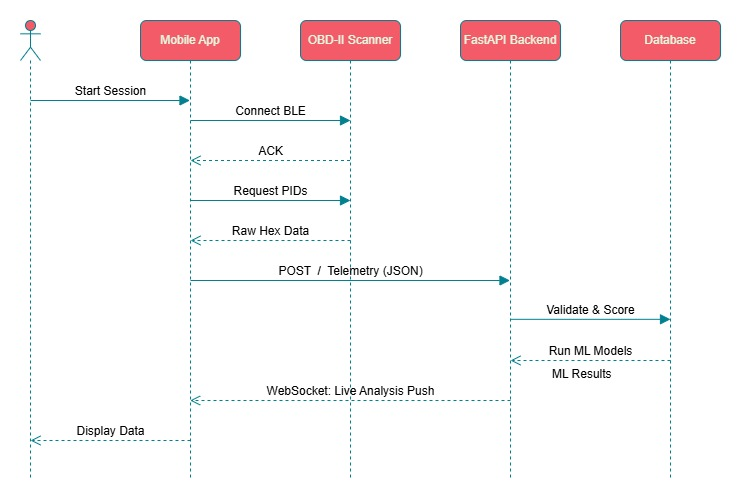
\includegraphics[width=0.6\textwidth]{SeqDiagram1.jpg}
\caption{Sequence 1: Real-Time Monitoring Session over WebSocket}
\end{figure}
\begin{figure}[H]
\centering
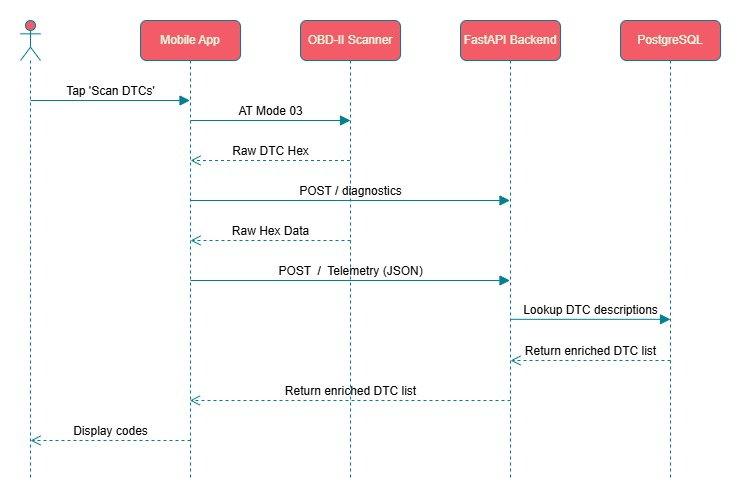
\includegraphics[width=0.6\textwidth]{SeqDiagram2.jpg}
\caption{Sequence 2: DTC Injection, Decoding \& Service Ticket Flow}
\end{figure}
\begin{figure}[H]
\centering
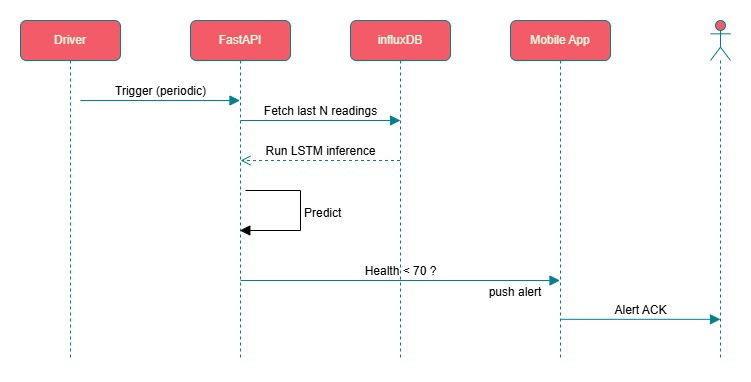
\includegraphics[width=0.6\textwidth]{SeqDiagram3.jpg}
\caption{Sequence 3: Rolling-Buffer ML Inference and Anomaly Alert}
\end{figure}
\subsection{Class diagram}
The class diagram models the core domain entities and their relationships within the AutoVue backend and Android application. Classes are organized into three packages: Data Acquisition Services, ML Components, and the Android client (ViewModels, repositories, and UI state).
\begin{figure}[H]
\centering
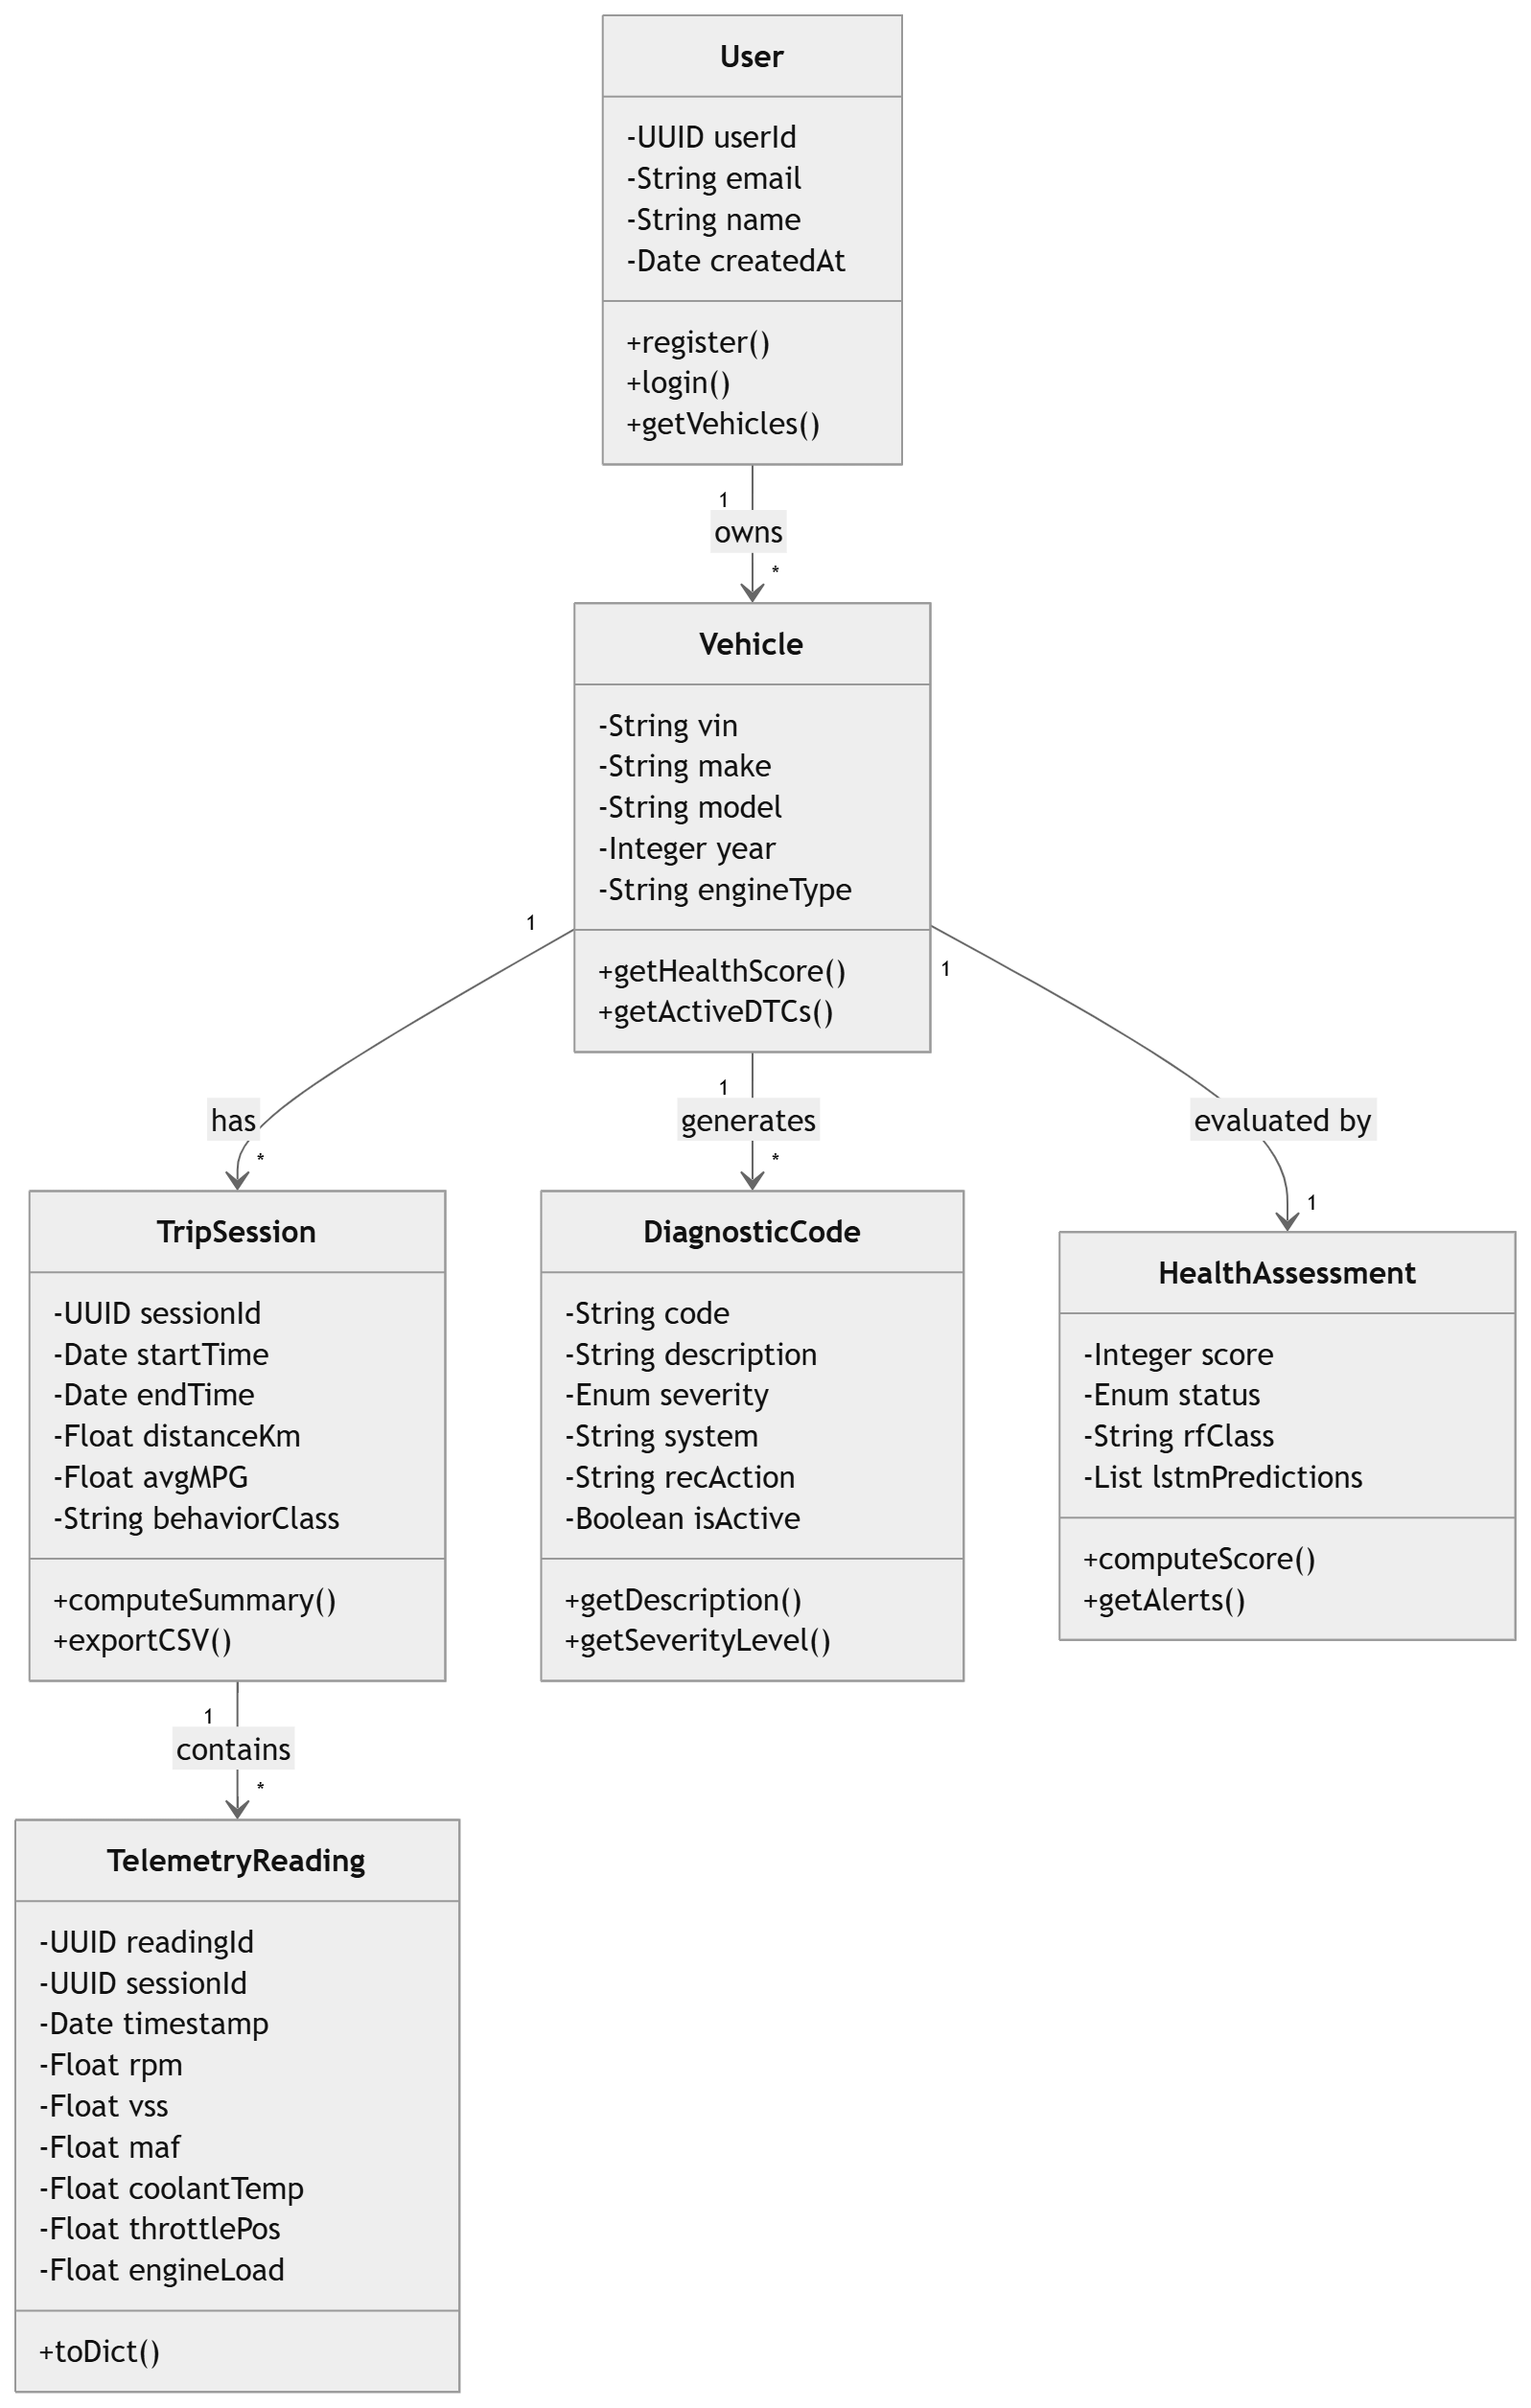
\includegraphics[width=0.6\textwidth]{mermaid-diagram.png}
\caption{Class 1: Core Domain class}
\end{figure}

\begin{figure}[H]
\centering
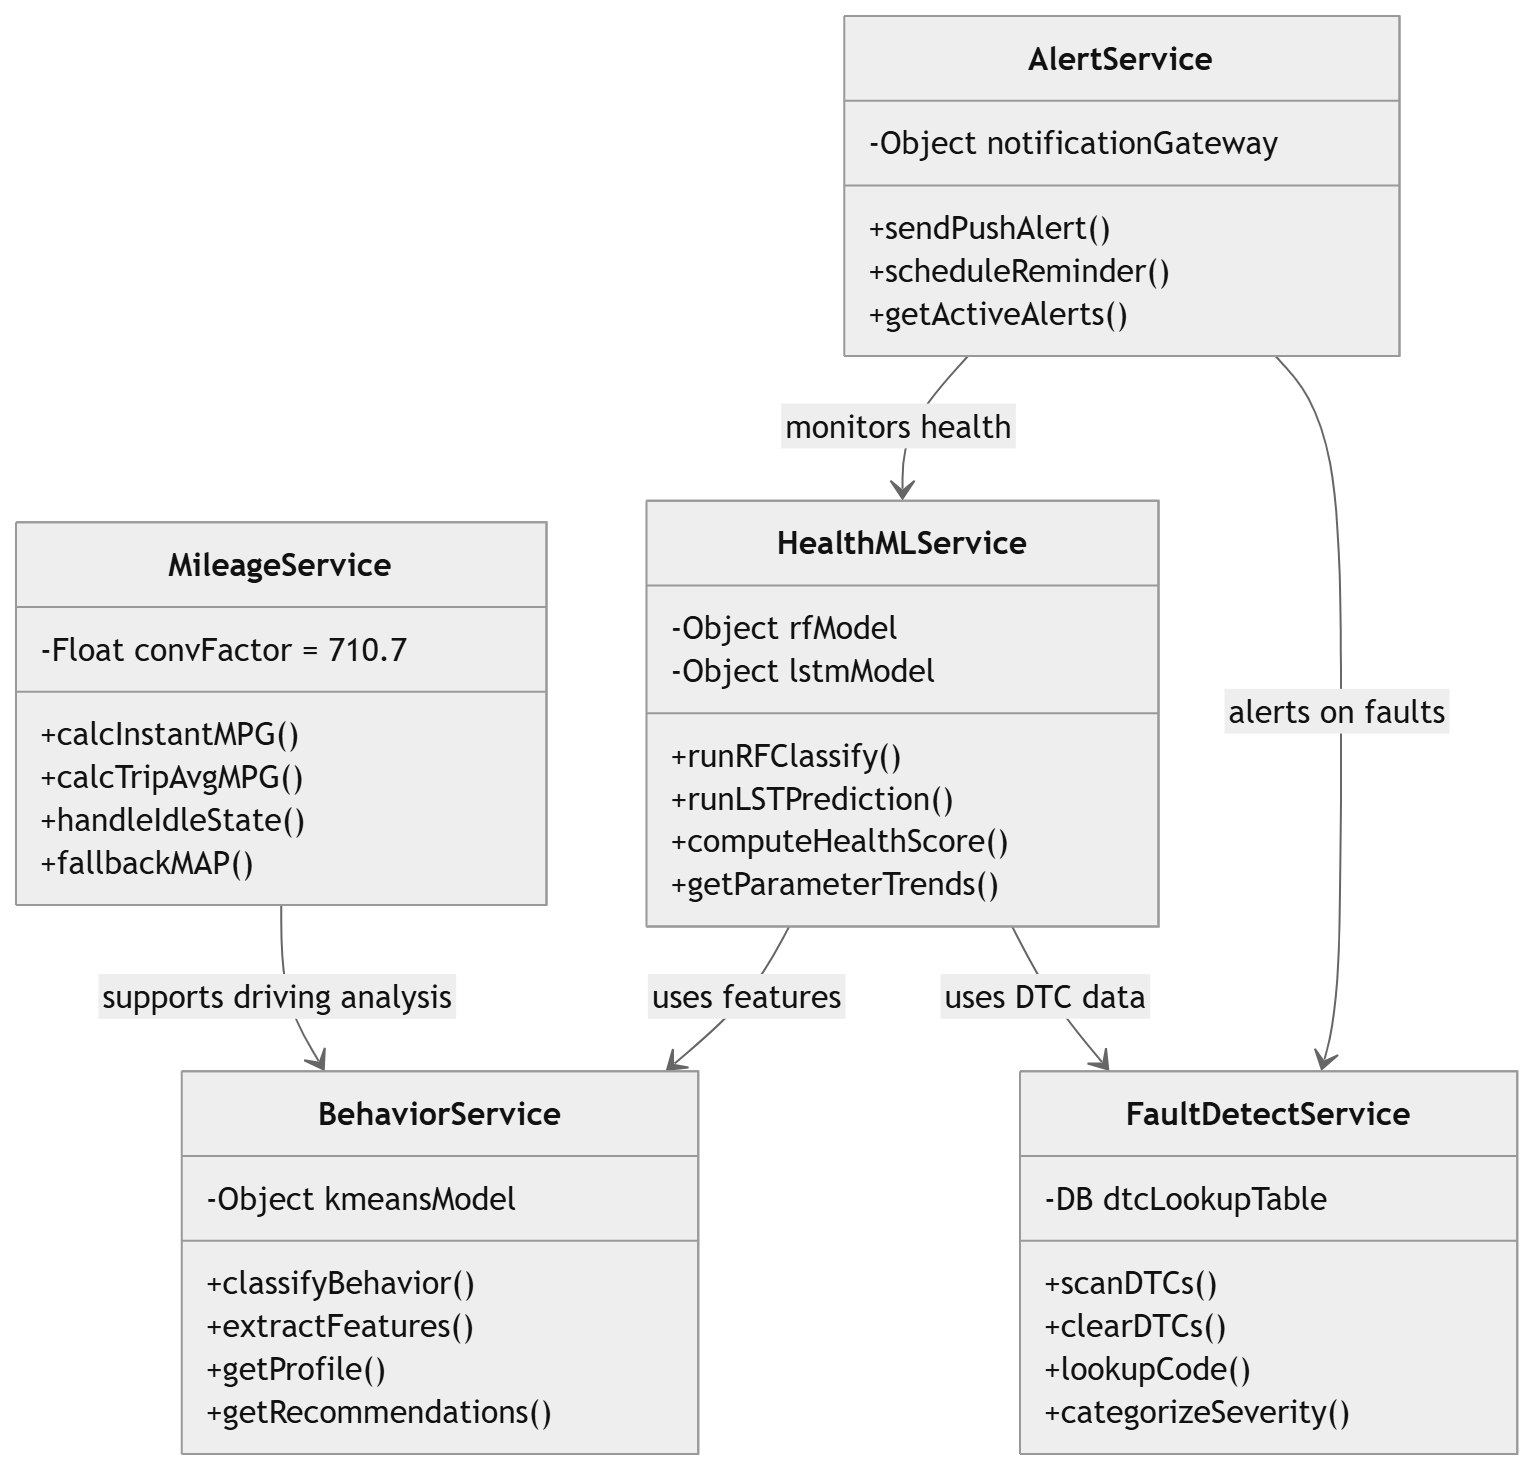
\includegraphics[width=0.8\textwidth]{class2.png}
\caption{Class 2: Service Layer Classes}
\end{figure}

\section{Control Flow Diagram}

The system processes vehicle data in a sequential flow. Live data is acquired directly from the ECU via Bluetooth, merged with DTC/GPS state, pushed into the rolling ML buffer, passed through the three inference functions, and broadcast to clients over WebSocket, while the Android client renders instrumentation and raises alerts.
\begin{figure}[H]
\centering
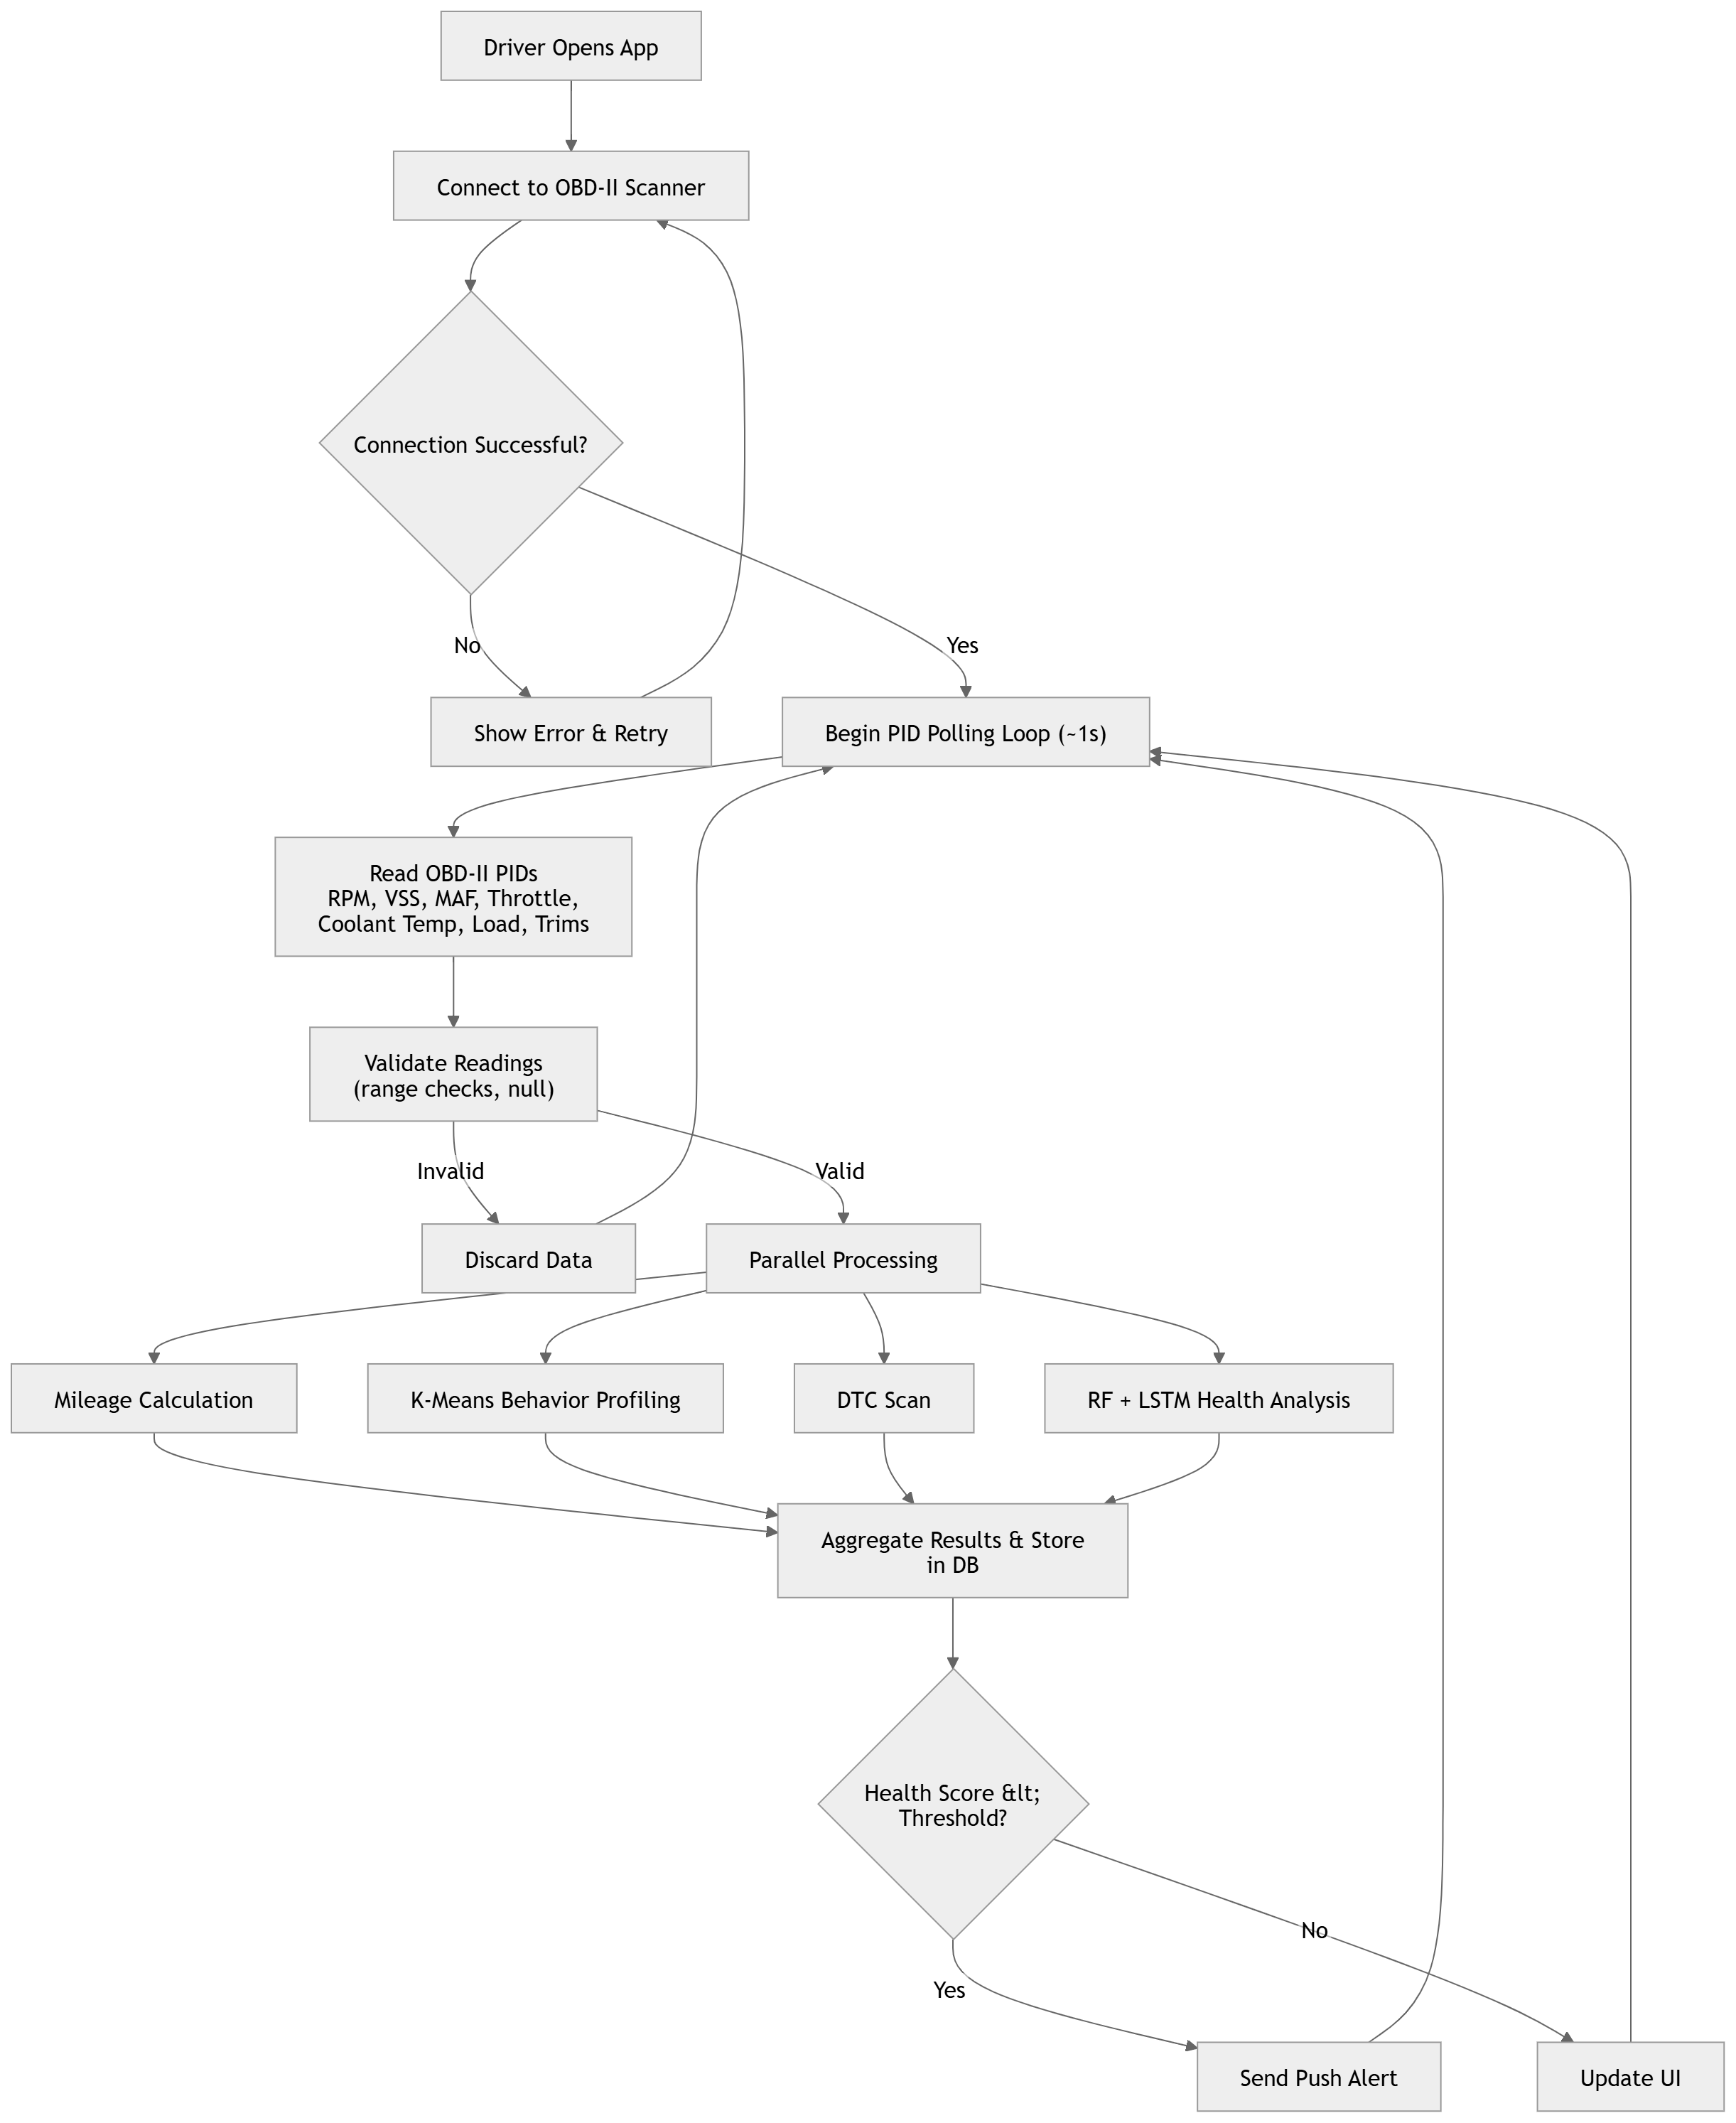
\includegraphics[width=1\textwidth]{control1.png}
\caption{Complete System Flow diagram}
\end{figure}

% \subsection{Algorithms for Logic Implementation}

% \begin{figure}[H]
% \centering
% 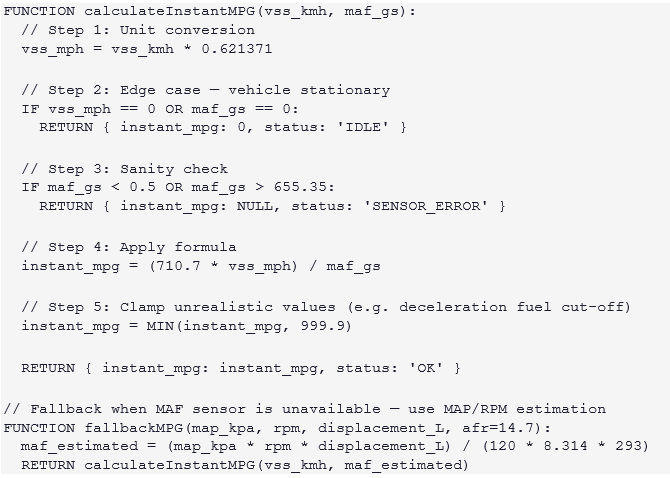
\includegraphics[width=1\textwidth]{alg1.png}
% \caption{Algorithm 1: Three-Tier Physics Fuel Estimation}
% \end{figure}

% \begin{figure}[H]
% \centering
% 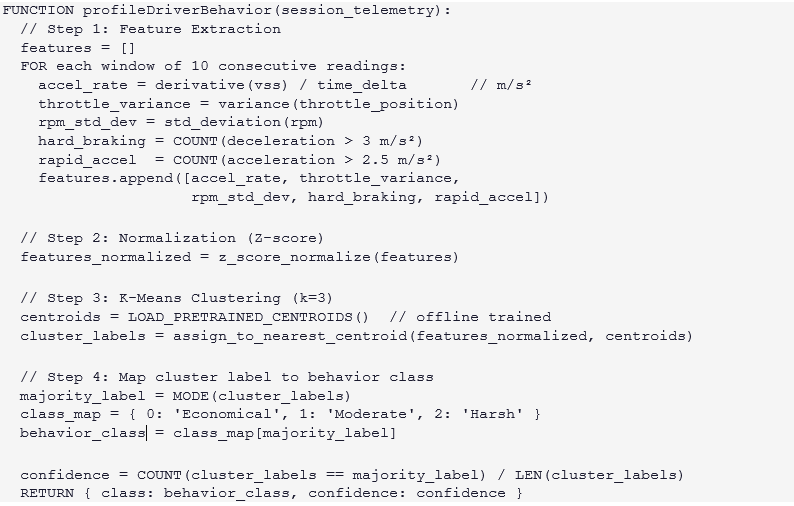
\includegraphics[width=1\textwidth]{alg2.png}
% \caption{Algorithm 2: XGBoost Driver Behaviour Feature Extraction and Classification}
% \end{figure}

% \begin{figure}[H]
% \centering
% 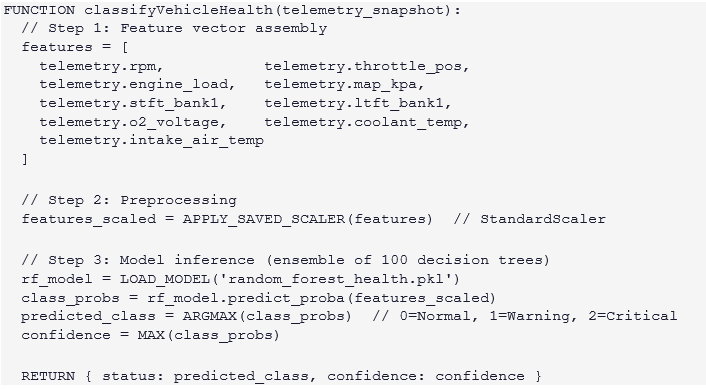
\includegraphics[width=1\textwidth]{alg3.png}
% \caption{Algorithm 3: LSTM Autoencoder Health Anomaly Detection}
% \end{figure}

% \begin{figure}[H]
% \centering
% 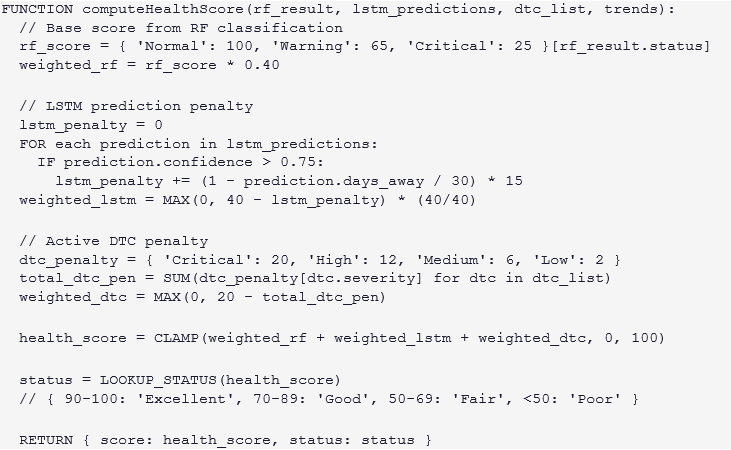
\includegraphics[width=1\textwidth]{alg4.png}
% \caption{Algorithm 4: Sensor Override Tick Merging and Release}
% \end{figure}

\subsection{Activity Diagram for Use Cases}

\begin{figure}[H]
\centering
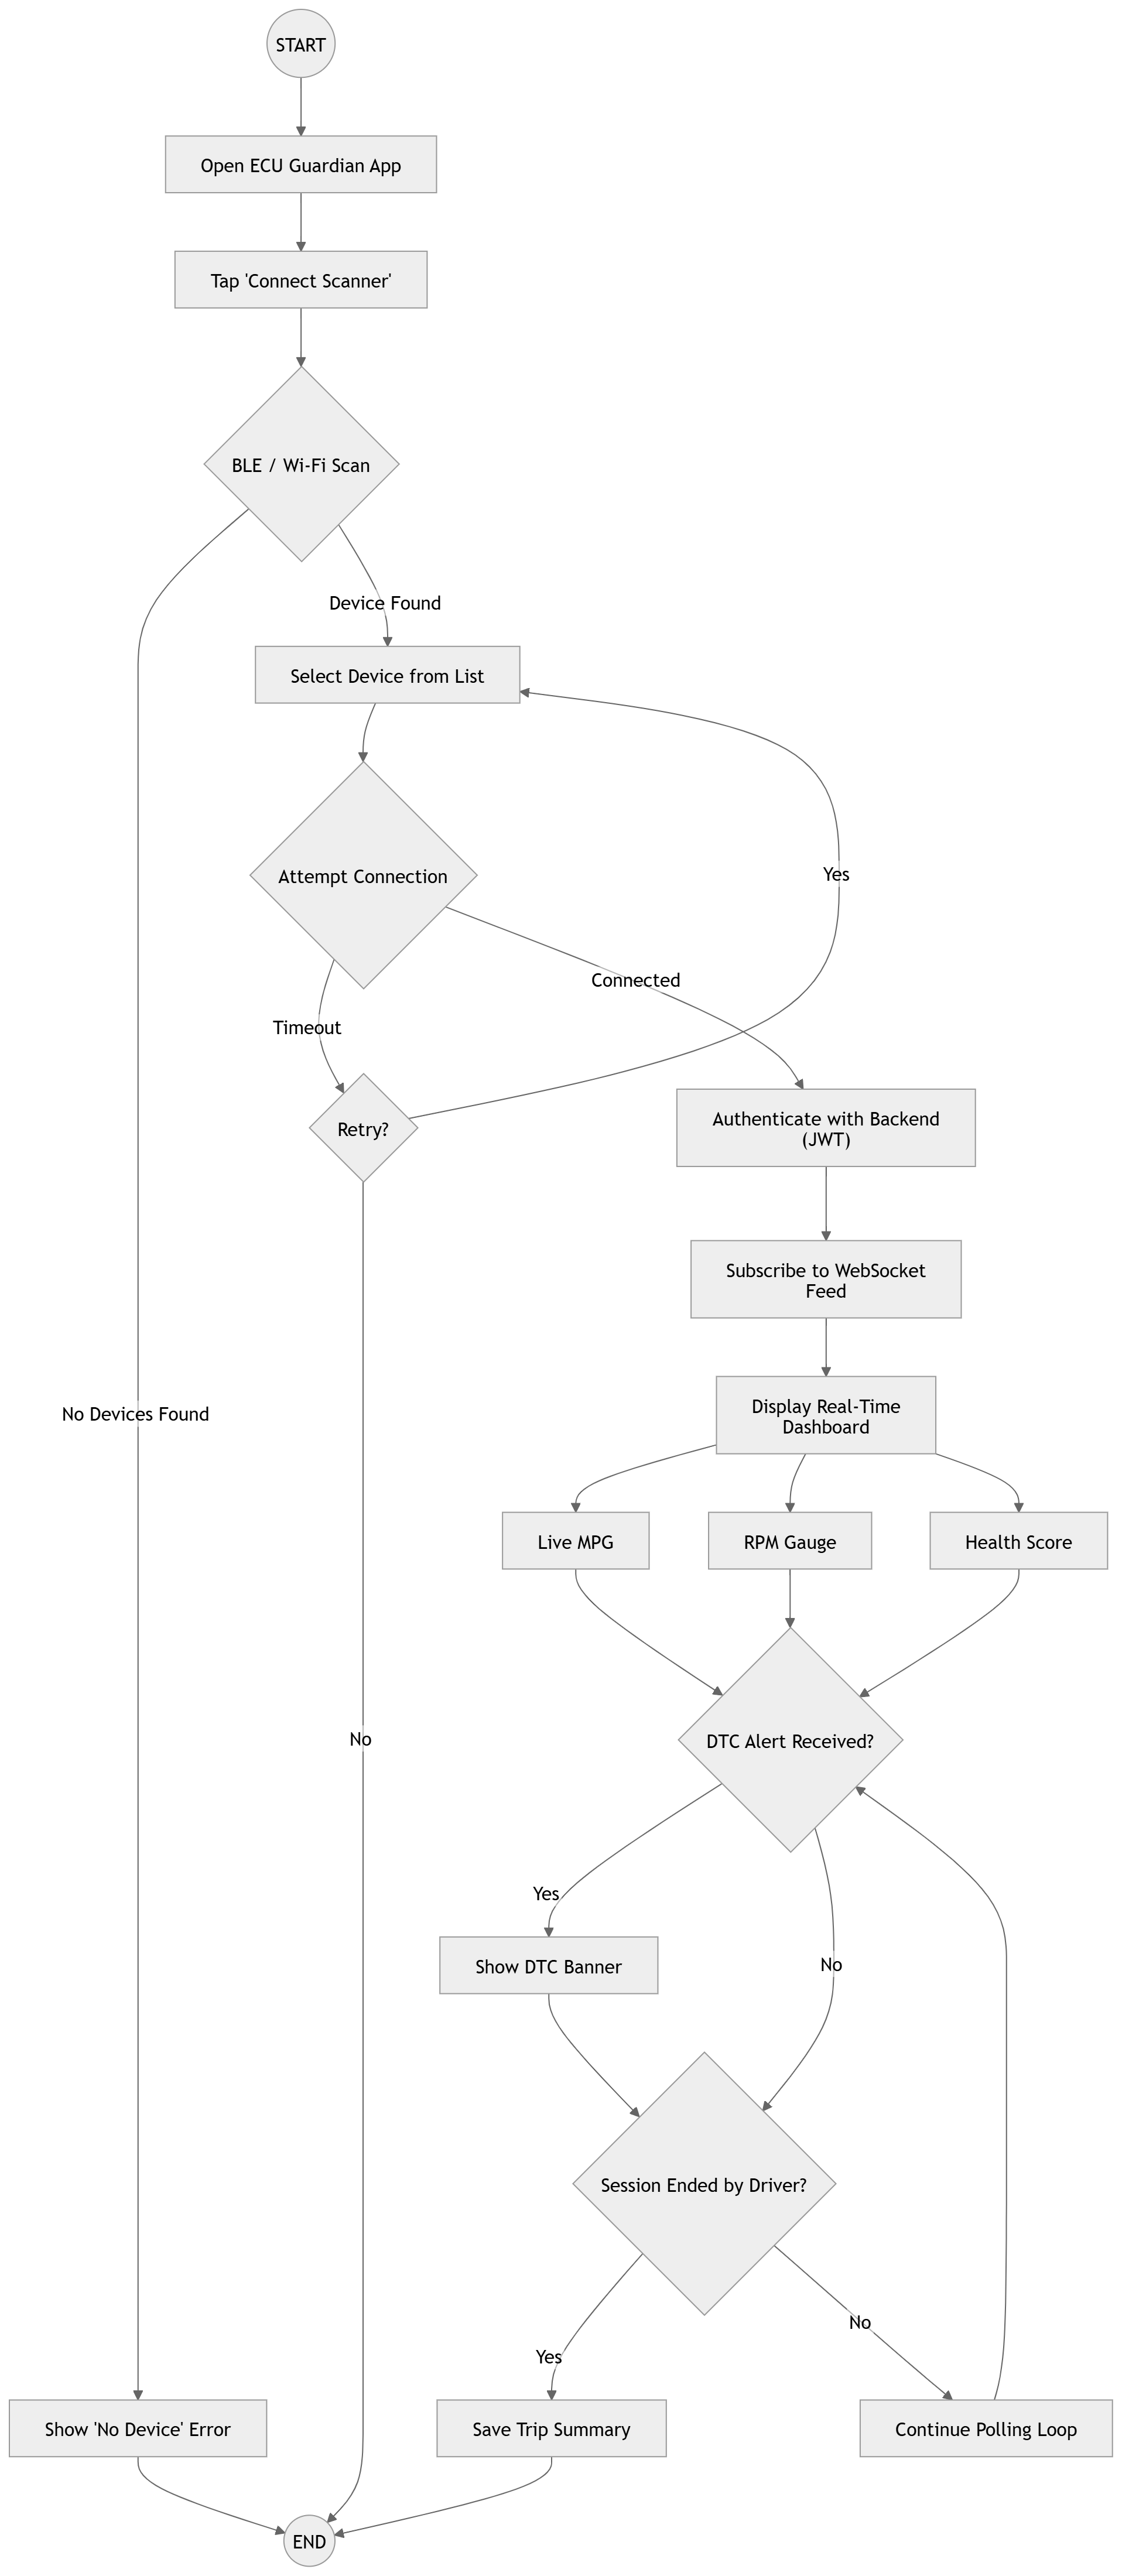
\includegraphics[width=0.63\textwidth]{act1.png}
\caption{Driver Connects and Views the Live Cockpit}
\end{figure}
\begin{figure}[H]
\centering
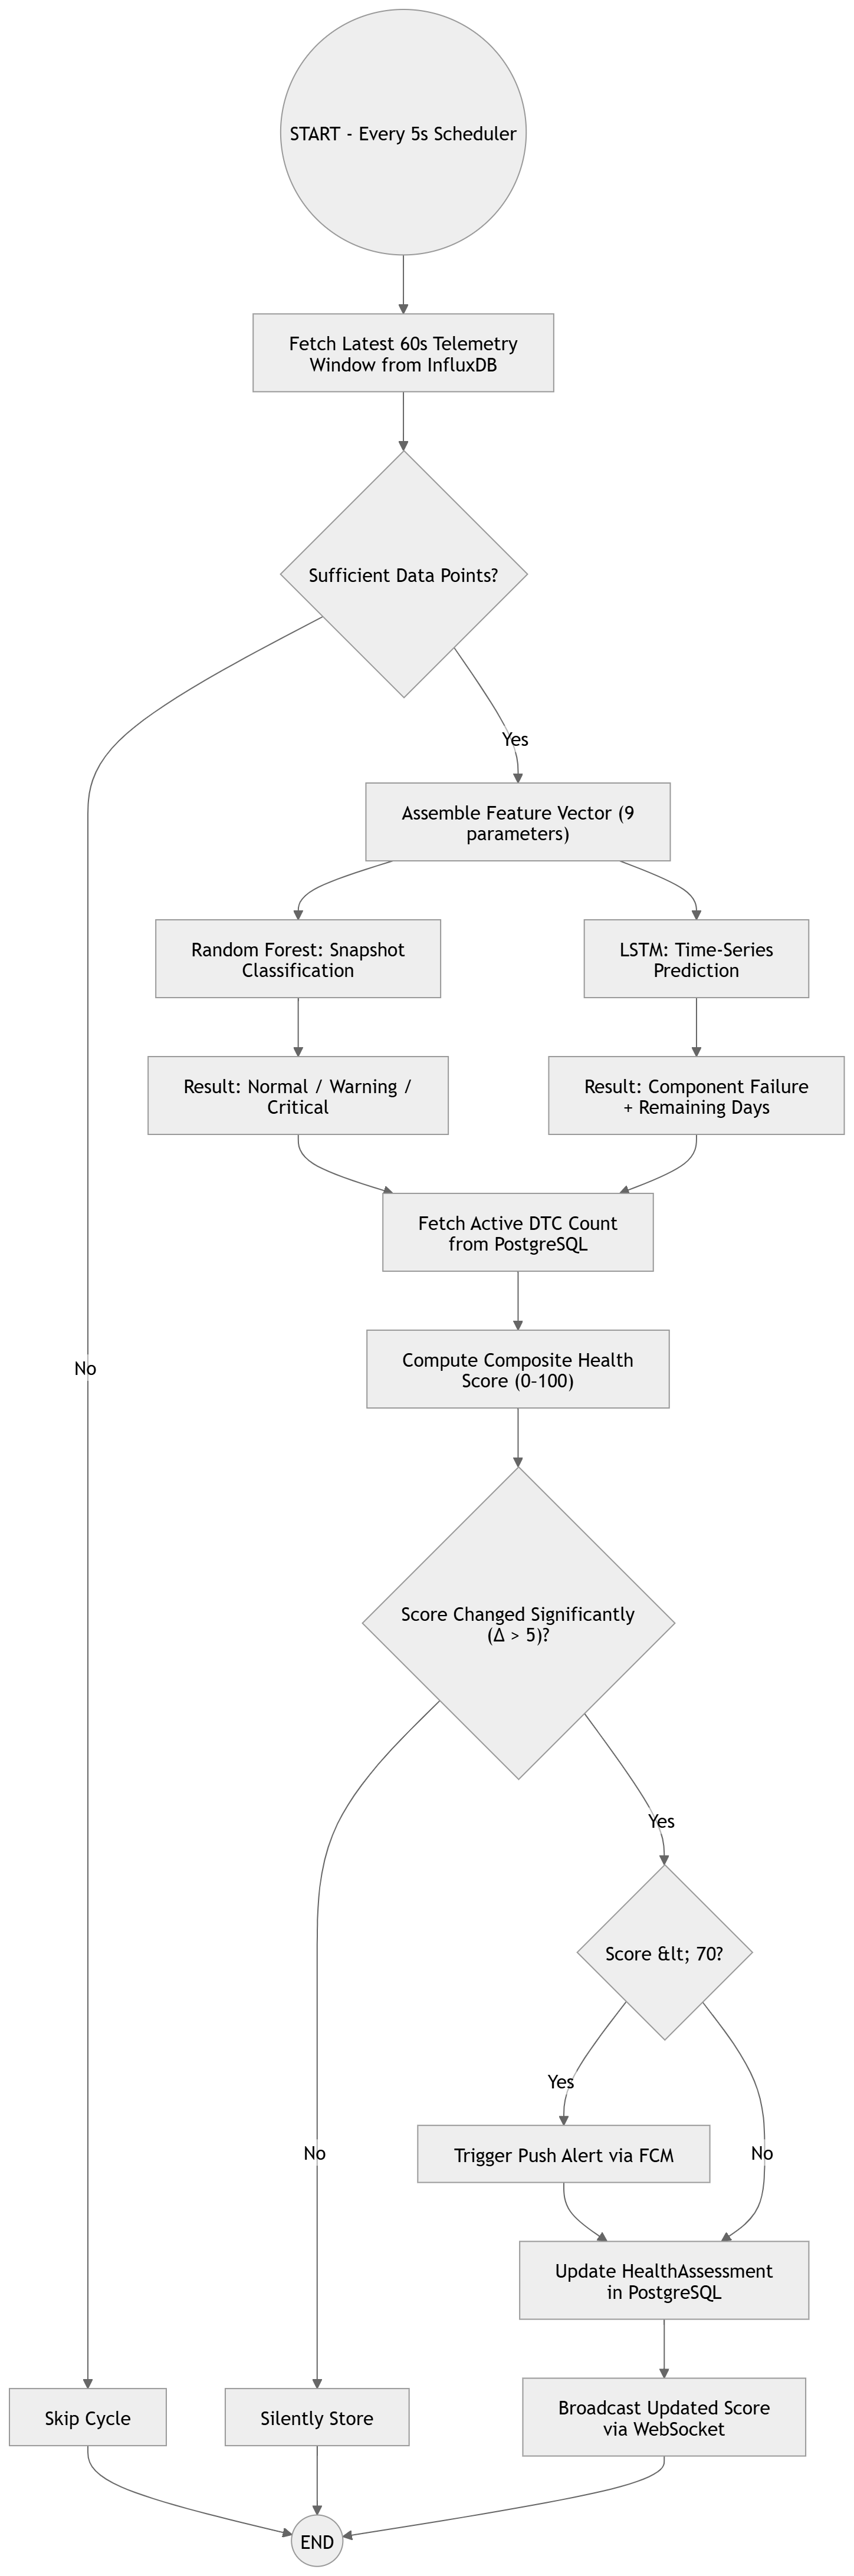
\includegraphics[width=0.5\textwidth]{act2.png}
\caption{Rolling-Buffer ML Health Monitoring Pipeline}
\end{figure}


%---------------------------- Chapter FIVE --------------------------

\chapter{Implementation}
\section{Introduction}

This chapter describes the practical realization of AutoVue, translating the architecture and design of Chapter 4 into working software. The implementation comprises two deliverables deployed as a unit: a single FastAPI backend process that combines the machine learning API with the real-time Bluetooth data gateway, and a native Android application built with Jetpack Compose that acts as the driver's cockpit. The gateway runs the three ML inference functions directly on a rolling buffer of incoming ticks, so every WebSocket message carries raw sensor data and fresh ML results in one push, with zero additional API calls from the client. \par

The implementation prioritises the standard ten-field sensor contract as the single interface between the vehicle's OBD-II stream, the ML models, and the clients. This is what allows physical ELM327 adapters to seamlessly drive the analytical engine without touching downstream code.

\section{Development Environment and Tools}

The system was developed and tested using the following environment:

\begin{table}[H]
\centering
\renewcommand{\arraystretch}{1.3}
\begin{tabular}{|p{4.5cm}|p{8.5cm}|}
\hline
\textbf{Component} & \textbf{Tool / Version} \\
\hline
Backend Language & Python 3.11 \\ \hline
Backend Framework & FastAPI 0.111 (Uvicorn) \\ \hline
ML Frameworks & XGBoost 2.0, PyTorch 2.2, Scikit-learn \\ \hline
Data Processing & NumPy, Pandas \\ \hline
Android Language & Kotlin (Coroutines, StateFlow) \\ \hline
Android UI & Jetpack Compose, Material Design 3 \\ \hline
Android Networking & OkHttp WebSocket client, Retrofit 2 + Moshi \\ \hline
Android Audio & Android Text-to-Speech engine \\ \hline
IDE & Android Studio, Visual Studio Code, Jupyter Notebook \\ \hline
Containerization & Docker (single-container deploy to Render) \\ \hline
Version Control & Git / GitHub \\ \hline
\end{tabular}
\caption{Development Environment and Tool Versions}
\end{table}

\section{OBD-II Data Acquisition and Streaming}

The Bluetooth data gateway is the backbone of the platform. It establishes a connection with a physical ELM327 OBD-II adapter, continuously polling the vehicle's ECU for standard PIDs, and normalises them onto the standard field contract. The acquisition engine reads these values in real-time, builds each tick, and hands it to the inference and broadcast stages. Listing~\ref{lst:sim} shows the core acquisition loop.

\begin{lstlisting}[language=Python, caption={Live Bluetooth Data Acquisition Engine (simplified)}, label={lst:sim}]
import asyncio
import obd

class DataAcquisitionGateway:
    def __init__(self, ml_buffer, broadcaster):
        self.connection = obd.Async() # connects to default Bluetooth/USB OBD
        self.ml_buffer = ml_buffer
        self.broadcaster = broadcaster
        self.state = "stopped"
        self.dtcs = []

    async def run(self):
        if not self.connection.is_connected():
            return
        self.state = "running"
        while self.state == "running":
            tick = self.build_tick()
            self.ml_buffer.append(tick["data"])
            tick["ml"] = self.ml_buffer.infer()   # driver/health/fuel
            await self.broadcaster.push(tick)
            await asyncio.sleep(1.0) # 1 Hz acquisition rate

    def build_tick(self):
        data = {k: float(self.query_pid(k)) for k in STANDARD_FIELDS}
        tick = {"data": data}
        if self.dtcs:
            tick["dtcs"] = list(self.dtcs)
        # GPS data acquired directly from Android device
        return tick

    def query_pid(self, field_name):
        # Maps standard fields to OBD commands
        cmd = self.map_to_obd_cmd(field_name)
        response = self.connection.query(cmd)
        return response.value.magnitude if not response.is_null() else 0.0
\end{lstlisting}

Unsupported or missing fields default to \texttt{0.0} rather than raising, satisfying the constraint that monitoring never fails because a vehicle lacks a particular PID.

\section{Rolling ML Buffer and Automatic Inference}

A bounded rolling buffer accumulates the most recent ticks. Each model activates at its own window size — fuel at 20 ticks, health at 24, driver behaviour at 30 — after which every broadcast carries a populated \texttt{ml} key. During the warm-up ticks the key is an empty object, which both clients treat as ``model not ready''. The buffer is the only coupling between the data acquisition gateway and the models: the models never know where data comes from.

\section{Driver Behaviour Classification (XGBoost)}

The driver model evaluates driving smoothness rather than absolute values. From each rolling window of RPM, speed, and throttle arrays it engineers nine features — window index, average speed, speed deviation, mean RPM, RPM standard deviation, mean pedal position, pedal standard deviation, maximum speed, and acceleration standard deviation — standardises them with a pickled scaler, and classifies the window as \textbf{Economical}, \textbf{Moderate}, or \textbf{Aggressive} with a confidence score and a coaching sentence drawn from the model metadata. Listing~\ref{lst:driver} shows the inference path.

\begin{lstlisting}[language=Python, caption={XGBoost Driver Behaviour Inference}, label={lst:driver}]
import joblib, numpy as np

class DriverBehaviourModel:
    def __init__(self, model_dir="models/"):
        self.model = joblib.load(model_dir + "driver_model.pkl")
        self.scaler = joblib.load(model_dir + "driver_scaler.pkl")
        meta = json.load(open(model_dir + "driver_metadata.json"))
        self.features = meta["features"]
        self.labels = meta["labels"]
        self.tts = meta["tts_messages"]

    def predict(self, rpm, speed, throttle, window_index=0):
        feats = {
            "window": window_index,
            "avg_speed": float(np.mean(speed)),
            "vs_dev": float(np.std(speed)),
            "mean_rpm": float(np.mean(rpm)),
            "rpm_std": float(np.std(rpm)),
            "mean_pedal": float(np.mean(throttle)),
            "pedal_std": float(np.std(throttle)),
            "max_speed": float(np.max(speed)),
            "accel_std": float(np.std(np.diff(speed))),
        }
        X = self.scaler.transform(
                [[feats[f] for f in self.features]])
        proba = self.model.predict_proba(X)[0]
        best = int(np.argmax(proba))
        return {"label": self.labels[best],
                "confidence": round(float(proba[best]), 4),
                "tts_message": self.tts[self.labels[best]],
                "feature_values": feats}
\end{lstlisting}

\section{Vehicle Health Anomaly Detection (LSTM Autoencoder)}

The health model learns the normal correlations among ten sensor features over 24-tick sequences. At inference, the reconstruction error per feature is compared against that feature's optimised threshold; if any feature exceeds its threshold the tick is flagged anomalous, and the features that fired are reported by name so the driver sees \emph{which} relationships broke, not just \emph{that} something broke. Listing~\ref{lst:health} shows the scoring logic.

\begin{lstlisting}[language=Python, caption={LSTM Autoencoder Anomaly Scoring}, label={lst:health}]
import torch, joblib
from app.ml.autoencoder import LSTMAutoencoder

class HealthModel:
    def __init__(self, model_dir="models/"):
        cfg = joblib.load(model_dir + "health_model_config.pkl")
        self.seq_len, self.cols = cfg["seq_len"], cfg["feature_cols"]
        self.net = LSTMAutoencoder(cfg["n_features"],
                                   cfg["hidden_dim"], cfg["latent_dim"])
        self.net.load_state_dict(
            torch.load(model_dir + "lstm_autoencoder.pt"))
        self.net.eval()
        self.scaler = joblib.load(model_dir + "health_scaler.pkl")
        self.thresholds = joblib.load(
            model_dir + "optimized_thresholds.pkl")

    def predict(self, ticks):
        seq = np.array([[t[c] for c in self.cols]
                        for t in ticks[-self.seq_len:]])
        seq = self.scaler.transform(seq)
        with torch.no_grad():
            recon = self.net(torch.tensor(seq).unsqueeze(0))[0].numpy()
        errors = np.mean((seq - recon) ** 2, axis=0)
        named = {label: round(float(e), 6)
                 for label, e in zip(self.cols, errors)}
        triggered = [label for label, e in named.items()
                     if e > self.thresholds.get(label, 0.05)]
        score = max(named.values()) if named else 0.0
        return {"is_anomaly": len(triggered) > 0,
                "status": "Anomaly" if triggered else "Normal",
                "anomaly_score": score,
                "feature_errors": named,
                "triggered_features": triggered}
\end{lstlisting}

\section{Fuel Consumption Estimation (Three-Tier Physics Engine)}

Fuel estimation deliberately requires no training. Tier 1 divides the Mass Air Flow by the stoichiometric air-fuel ratio (14.7) and converts to volume using the fuel density of BS6 E10 fuel (0.730 g/mL). Tier 2 applies the speed-density equation using MAP, RPM, intake temperature, and a volumetric-efficiency estimate. Tier 3 falls back to a throttle-and-RPM heuristic. Below 200 RPM the engine is treated as off. Instantaneous mileage is returned only when speed exceeds 2 km/h, and is capped at 50 km/L.

\begin{lstlisting}[language=Python, caption={Three-Tier Physics Fuel Estimator}, label={lst:fuel}]
AFR, FUEL_DENSITY = 14.7, 0.730      # g/mL, BS6 E10
DISPLACEMENT = 1.598                 # Seat Leon 1.6 FSI (litres)

def estimate_fuel(window):
    avg = {k: float(np.mean([t[k] for t in window])) for k in
           ("rpm", "vss", "maf", "map_kpa", "intake_air_temp",
            "throttle_pos")}
    if avg["rpm"] <= 200:
        return {"fcr_gs": 0.0, "mileage_kmpl": None, "tier": 0,
                "method": "stopped", "vss_kmph": avg["vss"]}
    if avg["maf"] > 0.5:
        fcr = avg["maf"] / AFR                     # Tier 1
        method = "maf"; tier = 1
    elif avg["map_kpa"] > 0:
        ve = 0.85                                  # Tier 2 speed-density
        air_g_s = (avg["map_kpa"] * DISPLACEMENT * ve
                   * avg["rpm"] / 120.0
                   / (273.15 + avg["intake_air_temp"]) * 2.697)
        fcr = air_g_s / AFR
        method = "map_rpm"; tier = 2
    else:                                          # Tier 3 heuristic
        fcr = 0.35 + avg["throttle_pos"] / 100.0 \
              * avg["rpm"] / 1000.0 * 2.0
        method = "throttle_heuristic"; tier = 3
    mileage = (avg["vss"] * FUEL_DENSITY * 1000.0
               / (fcr * 3600.0)) if avg["vss"] >= 2 else None
    return {"fcr_gs": round(fcr, 4),
            "mileage_kmpl": round(min(mileage, 50.0), 2)
                           if mileage else None,
            "method": method, "tier": tier,
            "vss_kmph": avg["vss"]}
\end{lstlisting}

\section{Backend API and WebSocket Layer}

REST endpoints expose the ML models directly (\texttt{/api/driver/predict}, \texttt{/api/health/predict}, \texttt{/api/fuel/predict}), serve snapshots and bounded history (\texttt{/api/live-data}, \texttt{/api/ml/latest}, \texttt{/api/history}), and handle DTCs and GPS routes. A WebSocket channel broadcasts live ticks. Listing~\ref{lst:ws} shows the connection manager and live-tick broadcast.

\begin{lstlisting}[language=Python, caption={WebSocket Broadcast Layer}, label={lst:ws}]
from fastapi import FastAPI, WebSocket, WebSocketDisconnect

app = FastAPI(title="AutoVue Backend")
manager = ConnectionManager()          # active /api/ws/live clients

@app.websocket("/api/ws/live")
async def ws_live(ws: WebSocket):
    await manager.connect(ws)
    try:
        while True:
            await ws.receive_text()    # keepalive; ticks are pushed
    except WebSocketDisconnect:
        manager.disconnect(ws)

async def on_tick(tick):
    await manager.broadcast(tick)      # called by the data gateway

@app.get("/api/live-data")
def live_data():
    gw = gateway.status()
    if gw["state"] == "stopped":
        raise HTTPException(404, "Data acquisition not started")
    return {"data": gateway.last_tick["data"],
            "ml": gateway.last_tick.get("ml", {})}
\end{lstlisting}

\section{DTC Management}

DTC endpoints maintain an active fault list acquired from the vehicle's ECU, which appears in every tick as a \texttt{dtcs} array and is omitted entirely when empty, allowing the driver to clear or review historical faults directly from the cockpit.

\section{GPS Route Integration}

Live GPS coordinates are acquired from the Android device running the cockpit application. Latitude, longitude, elevation, bearing, and speed are polled and seamlessly fused with the incoming OBD-II telemetry in real-time. The backend serves the full polyline through \texttt{/api/route} and aggregated statistics through \texttt{/api/trip-summary}, and each tick carries its position so the Android map animates dynamically during the drive.

\section{Android Application}

The Android client is a single-activity Jetpack Compose application organised in Clean Architecture / MVVM. A manual dependency container (\texttt{AppContainer}) wires the configurable base URL, the OkHttp WebSocket client with automatic REST polling fallback, Retrofit services, and the Text-to-Speech engine. State flows drive the UI: the cockpit screen renders custom canvas analog gauges (sweep-needle speedometer, tachometer with redline, temperature zones, fuel meter) and a trip HUD computing distance, cost, average consumption, and an eco-driving score; a sensor grid and a multi-channel scrolling oscilloscope visualise the live stream; an alert engine with severity tags (CRITICAL, WARNING, INFO) and spoken announcements with per-category toggles and cooldown debounce raises overspeed, overheat, cold-rev, and anomaly alerts; DTC scanning feeds a decoder with symptom explanations and a digital service-ticket creator stamped with VIN, mileage, and fault description; and the trip module renders GPS heatmaps (speed, behaviour, efficiency overlays), a refuelling diary, and the start-stop efficiency tracker. A two-page onboarding wizard captures the vehicle and driver profile parameters that calibrate the physics fuel model, and multiple profiles can be registered and switched.

\section{Integration and Deployment}

The entire backend ships as one Docker container deployable to Render's free tier, or can be run locally via a Raspberry Pi directly hooked to the vehicle. During integration testing the full chain — real vehicle sensor to gauge needle, including all three ML models — was verified end-to-end over both WebSocket and REST fallback while connected to an actual car.

%------------ Chapter SIX --------------------------


\chapter{System Testing}
\section{Introduction}

System testing validates AutoVue end-to-end against the behaviours defined in the SRS: telemetry streaming, simulator playback control, the three ML models, override dials, DTC management, and GPS integration. Testing was performed against the deployed backend using its REST endpoints, WebSocket channels, the built-in control dashboard, and the Android application. Because the simulator is deterministic and dataset-driven, every test is reproducible without a vehicle.

\section{Test Environment}

\begin{table}[H]
\centering
\renewcommand{\arraystretch}{1.3}
\begin{tabular}{|p{4.5cm}|p{8.5cm}|}
\hline
\textbf{Item} & \textbf{Configuration} \\
\hline
Backend & FastAPI service, Docker container on Render free tier \\
\hline
Datasets & Bundled normal dataset (30{,}817 rows, $\approx$51 min) and bundled anomaly dataset \\
\hline
Clients & Built-in control dashboard, Android application (target SDK 34) \\
\hline
Transport & WebSocket (\texttt{wss://}) with REST polling fallback \\
\hline
\end{tabular}
\caption{Test Environment}
\end{table}

\section{Functional Test Cases}

\begin{table}[H]
\centering
\renewcommand{\arraystretch}{1.3}
\small
\begin{tabularx}{\textwidth}{|l|X|X|l|}
\hline
\textbf{ID} & \textbf{Test Case} & \textbf{Expected Result} & \textbf{Status} \\ \hline
TC01 & Start playback with default dataset & Streaming begins from row 0; status returns \texttt{running} & Pass \\ \hline
TC02 & Pause and resume playback & Tick broadcast halts on pause and continues from the same row on resume & Pass \\ \hline
TC03 & Change playback speed to each of 0.5x, 2x, 5x, 10x & Tick interval scales accordingly; invalid speeds rejected with 400 & Pass \\ \hline
TC04 & Stop and reset playback & Playback task cancelled; buffer cleared; row rewound to 0 & Pass \\ \hline
TC05 & Switch dataset during playback & Playback restarts from row 0 on the new dataset & Pass \\ \hline
TC06 & Upload, rename, and delete a dataset & Upload returns row/missing-value metadata; rename and delete succeed; bundled datasets protected from disk deletion & Pass \\ \hline
TC07 & Connect to \texttt{/api/ws/live} & One tick per simulated second, each with \texttt{data} and, after warm-up, \texttt{ml} & Pass \\ \hline
TC08 & Poll \texttt{/api/live-data} with simulator stopped & HTTP 404 returned; client falls back gracefully & Pass \\ \hline
TC09 & Observe \texttt{ml} key during first 30 ticks & \texttt{\{\}} until tick 20; fuel only from tick 20; health from tick 24; driver from tick 30 & Pass \\ \hline
TC10 & POST \texttt{/api/driver/predict} with $\geq$5 points & Returns label, confidence, TTS message, and 9 feature values & Pass \\ \hline
TC11 & POST \texttt{/api/health/predict} with $<$24 ticks & HTTP 400 & Pass \\ \hline
TC12 & POST \texttt{/api/fuel/predict} with 20+ ticks & Returns \texttt{fcr\_gs}, \texttt{mileage\_kmpl}, \texttt{method}, \texttt{tier} & Pass \\ \hline
TC13 & Set override dial on RPM and coolant & Tick \texttt{data} shows fixed values; \texttt{dataset\_data} honest; \texttt{overrides} lists both fields & Pass \\ \hline
TC14 & Release one dial, then all dials & Released fields snap back to dataset values on the next tick & Pass \\ \hline
TC15 & Inject DTCs \texttt{p0300}, \texttt{u0100} & Codes uppercased in \texttt{dtcs} array; key omitted after clearing & Pass \\ \hline
TC16 & Load GPS-enriched dataset; call \texttt{/api/route}, \texttt{/api/trip-summary} & Polyline, bounding box, distance and OBD statistics returned; non-GPS dataset returns 404 and the app hides the map & Pass \\ \hline
TC17 & Anomaly dataset playback & LSTM autoencoder flags anomaly with per-feature errors and triggered features & Pass \\ \hline
TC18 & Android alert engine & Overheat ($>$100\,\textdegree{}C) and cold-rev alerts fire with TTS; toggles and debounce respected & Pass \\ \hline
\end{tabularx}
\caption{Functional Test Results}
\end{table}

\section{Integration and Performance Testing}

The complete chain — dataset row, dial merging, rolling-buffer inference, WebSocket broadcast, and gauge rendering on the Android device — was verified under all playback speeds up to 10x, with inference completing within each tick interval. WebSocket reconnection and REST fallback were tested by interrupting connectivity mid-stream: the application resumed rendering from snapshot polling and re-attached to the live stream when the connection returned, with no loss of chart continuity on non-overridden channels. Free-tier cold-start behaviour was characterised and accounted for in demonstrations by warming the service in advance.

%---------------------------- Chapter SEVEN --------------------------
\chapter{Results and Discussion}
\section{Introduction}

This chapter presents the observed behaviour of the three machine learning models and the simulator features on the bundled datasets, using responses captured from the running system.

\section{Driver Behaviour Classification}

Over the normal driving dataset the XGBoost model produces stable rolling classifications. A representative idle-to-cruise window yields a \textbf{Moderate} classification with confidence 0.5035, the engineered features (average speed 19.71 km/h, RPM standard deviation 262.83, acceleration standard deviation 0.183), and the coaching message \emph{``Your driving is acceptable. Watch your speed variations and try to accelerate more gently.''} Smooth steady-speed windows shift the label toward \textbf{Economical} with high confidence, and the accompanying TTS coaching message confirms that the model responds to variance in speed, RPM, and pedal position rather than absolute magnitudes.

\section{Vehicle Health Anomaly Detection}

On normal data the LSTM Autoencoder reports \texttt{is\_anomaly: false} with reconstruction errors on the order of $10^{-6}$ across all ten features. Playing the bundled anomaly dataset drives per-feature errors above their optimised thresholds: a representative anomalous window reports \texttt{is\_anomaly: true} with an anomaly score of 3.9457 dominated by \textit{Engine RPM} (3.9457), followed by \textit{Air Flow Rate from Mass Flow Sensor} (0.8608) and \textit{Vehicle Speed Sensor} (0.2315) — exactly the signature of a sensor relationship breaking rather than a single value leaving range. Reporting errors per feature and by name is what makes the alert actionable, and it is this mechanism that powers the CRITICAL anomaly banner and spoken alert in the Android cockpit.

\section{Fuel Consumption Estimation}

On typical cruise conditions (45 km/h, 1500 RPM, MAF 12.5 g/s) the estimator selects Tier 1 (MAF-based) and returns a consumption rate of 1.23 g/s with an instantaneous mileage of 14.2 km/L. When MAF is absent, the speed-density Tier 2 engages; when only throttle and RPM are available, the Tier 3 heuristic bounds the estimate. Below 200 RPM the engine-off Tier 0 returns zero consumption, and below 2 km/h mileage is withheld rather than reported as a misleading figure. The transparency of the method — the response names the tier and method used — makes the output auditable in a way a black-box regressor is not.

\section{Simulator Feature Validation}

The override dials proved effective for live demonstration: pinning RPM at 5000 while the dataset reads 900 flows through the entire pipeline within one tick, the health model flags the broken RPM/airflow correlation, the alert banner fires, and releasing the dial restores the dataset trace with no restart. DTC injection and clearing behave per specification, and GPS replay produces a smooth route with heatmap overlays on the Android map.

\section{Discussion}

The results support the central design decisions of the project. Boosted trees proved the right tool for tabular driver classification; the reconstruction-based health model detects faults that single-sensor thresholds cannot, without requiring any labelled failure data; and a physics-first fuel estimator delivers plausible, explainable numbers with zero retraining. The simulator-first architecture made all of this testable, demonstrable, and reproducible — and because every layer speaks the same ten-field contract, the platform is positioned to accept live ELM327 data as a drop-in replacement for dataset playback.


\chapter{Conclusion and Future work}
\section{Conclusion}

This project set out to build an intelligent vehicle telemetry and diagnostics platform that transforms raw OBD-II data into actionable, driver-facing insight — and to make that platform demonstrable without requiring a physical vehicle at every step. The delivered system, AutoVue, achieves both goals. A single deployable FastAPI backend integrates three production machine learning models — an XGBoost driver behaviour classifier, a PyTorch LSTM Autoencoder health anomaly detector, and a three-tier physics-based fuel estimator — with an OBD-II simulator that streams real recorded driving data row by row over WebSocket and REST. A native Android cockpit renders that stream as analog-digital instrumentation, multi-channel oscilloscopes, GPS trip mapping, and spoken alerts, while a browser dashboard administers playback and provides the sensor override dials that make live fault injection reproducible. \par

Validation on bundled normal and anomaly datasets confirms that the health model flags broken sensor correlations before they become failures, that the driver model classifies on smoothness rather than raw magnitudes, and that the fuel engine produces auditable, tier-labelled estimates. The strict ten-field sensor contract throughout the stack is the project's key architectural decision: it is what makes datasets interchangeable, what will allow a physical ELM327 adapter to replace the simulator without touching downstream code, and what keeps the entire system honest to the OBD-II standard that consumer vehicles already speak.

\section{Future work}

The following extensions are identified on the project roadmap and follow naturally from the current architecture:
\begin{itemize}
  \item \textbf{Composite Vehicle Health Score (0--100):} a weighted aggregation of anomaly scores, DTC severity, and parameter deviations, building on the per-feature errors the LSTM Autoencoder already produces.
  \item \textbf{Predictive maintenance and Remaining Useful Life forecasting:} regression-based estimation of component lifetime to move the system from anomaly flagging to failure forecasting.
  \item \textbf{Persistent storage and authentication:} PostgreSQL-backed history and user accounts with JWT and bcrypt, replacing the current stateless, single-user prototype.
  \item \textbf{Real-time mobile push notifications} for critical anomalies, complementing the in-app banner and TTS alerts.
  \item \textbf{Live ELM327 acquisition adapter:} a sibling tick producer implementing the same field contract via the python-OBD library, graduating the platform from simulated to real vehicles.
\end{itemize}

\pagestyle{plain}
\renewcommand{\bibname}{References}

\addcontentsline{toc}{chapter}{References}

\printbibliography




\appendix

\chapter{Screenshots}

\begin{figure}[htp]
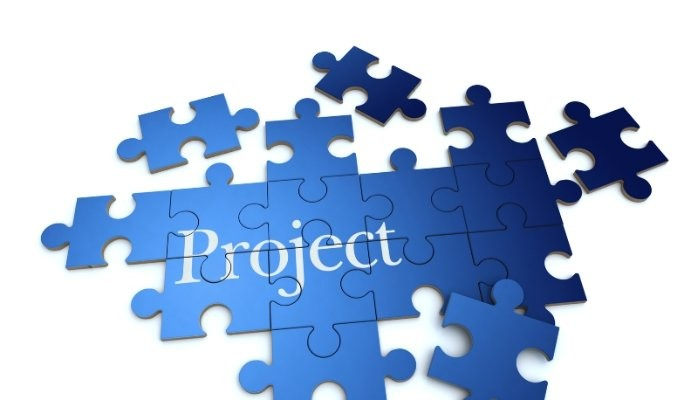
\includegraphics[width=5in,height=3in]{./pic/sample.jpg}
  \caption{AutoVue Android cockpit: analog-digital instrument cluster with trip computer HUD.}
  \label{figa1}
\end{figure}

\begin{figure}[htp]
    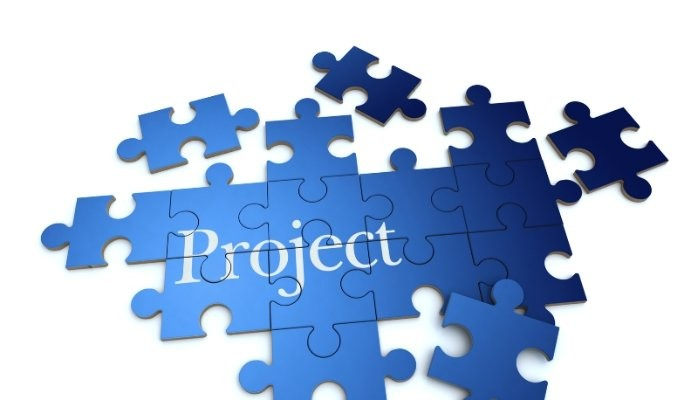
\includegraphics[width=5in,height=3in]{./pic/sample.jpg}
  \caption{Live telemetry sensor grid with OBD-II protocol and PID/s throughput.}
  \label{figa2}
\end{figure}

\begin{figure}[htp]
    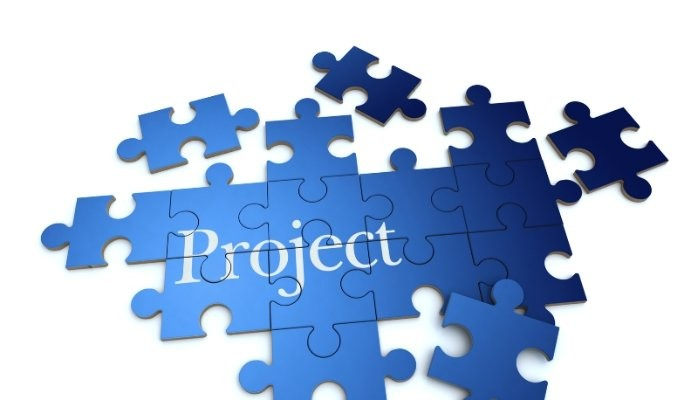
\includegraphics[width=5in,height=3in]{./pic/sample.jpg}
  \caption{Multi-channel oscilloscope waveform visualizer during playback.}
  \label{figa3}
\end{figure}

\begin{figure}[htp]
    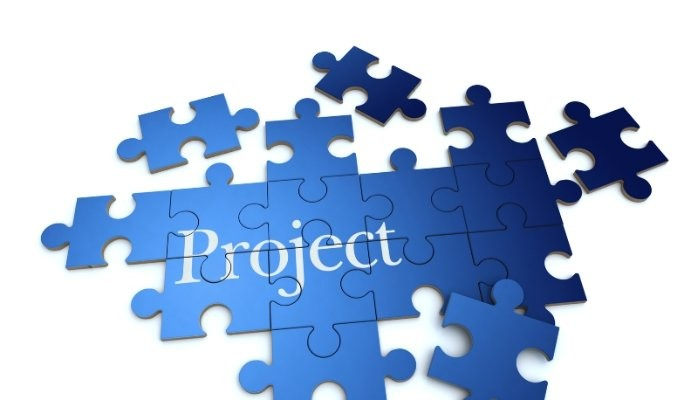
\includegraphics[width=5in,height=3in]{./pic/sample.jpg}
  \caption{Simulator control dashboard with sensor override dials.}
  \label{figa4}
\end{figure}

\begin{figure}[htp]
    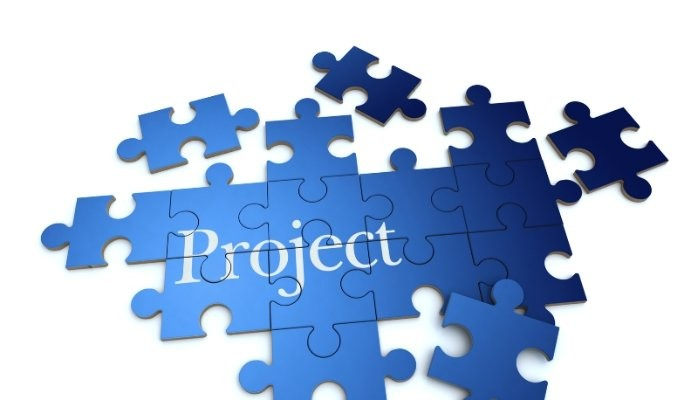
\includegraphics[width=5in,height=3in]{./pic/sample.jpg}
  \caption{GPS trip map with speed heatmap overlay and refuelling diary.}
  \label{figa5}
\end{figure}

\chapter{User Manual}

\section{Getting Started (Backend)}
\begin{enumerate}
  \item Clone the repository and install dependencies with \texttt{pip install -r requirements.txt} (Python 3.11).
  \item Start the service with \texttt{python run.py} (or \texttt{uvicorn app.main:app --reload --port 8000}). The bundled dataset loads automatically.
  \item Open the simulator control dashboard at \texttt{http://localhost:8000}, or the interactive API docs at \texttt{/docs}.
\end{enumerate}
For deployment, push to GitHub and create a Render Web Service from the included Dockerfile; warm the free-tier instance a few minutes before a live demo.

\section{Android Application}
\begin{enumerate}
  \item Build and install the app in Android Studio (target SDK 34) on a physical device or emulator.
  \item On first launch, complete the two-page profile wizard: profile name, fuel type, start-stop status, displacement, max power, odometer, curb weight, reference consumption, corrective factor, tank capacity, fuel level, and VIN. Multiple profiles can be registered and switched later.
  \item Tap \textbf{OBD Link} in the top bar to connect to the telemetry stream, or choose a simulation dataset from the backend.
  \item Use the cockpit for live gauges and trip statistics; the sensor grid and oscilloscope for raw telemetry; the alerts panel to configure TTS announcements and cooldowns; the DTC scanner to decode fault codes and create service tickets; the map for trip replay and refuelling entries; and the start-stop screen for idle savings.
\end{enumerate}

\section{Simulator Operations (Web Dashboard)}
\begin{enumerate}
  \item Select a dataset from the list (normal or anomaly session) and press \textbf{Start}; control playback with Pause, Resume, Stop, Reset, speed multipliers (0.5x--10x), and Loop.
  \item Activate a dial's checkbox and turn the knob to override a sensor (e.g., RPM 5000 or coolant 110\,\textdegree{}C); release the checkbox to snap back to the dataset instantly.
  \item Inject fault codes via the DTC panel to exercise the scanner and service-ticket flow on the Android app.
\end{enumerate}

\end{document}.l 